\chapter{Experiment}
\label{ch:part1}


\section{Microwave Model}

To analyze the properties of a ring resonator, a scaled microwave model is used. The setup is shown in Figure \ref{fig:setup}\footnote[1]{Jingshi Li, Materials for the preparation of Experiment 6}. The transmission through this waveguide structure (|$S_{21}$|) is analyzed with a network analyser (NWA). For each measurement the NWA was calibrated without the resonator 
\begin{figure}%
\centering
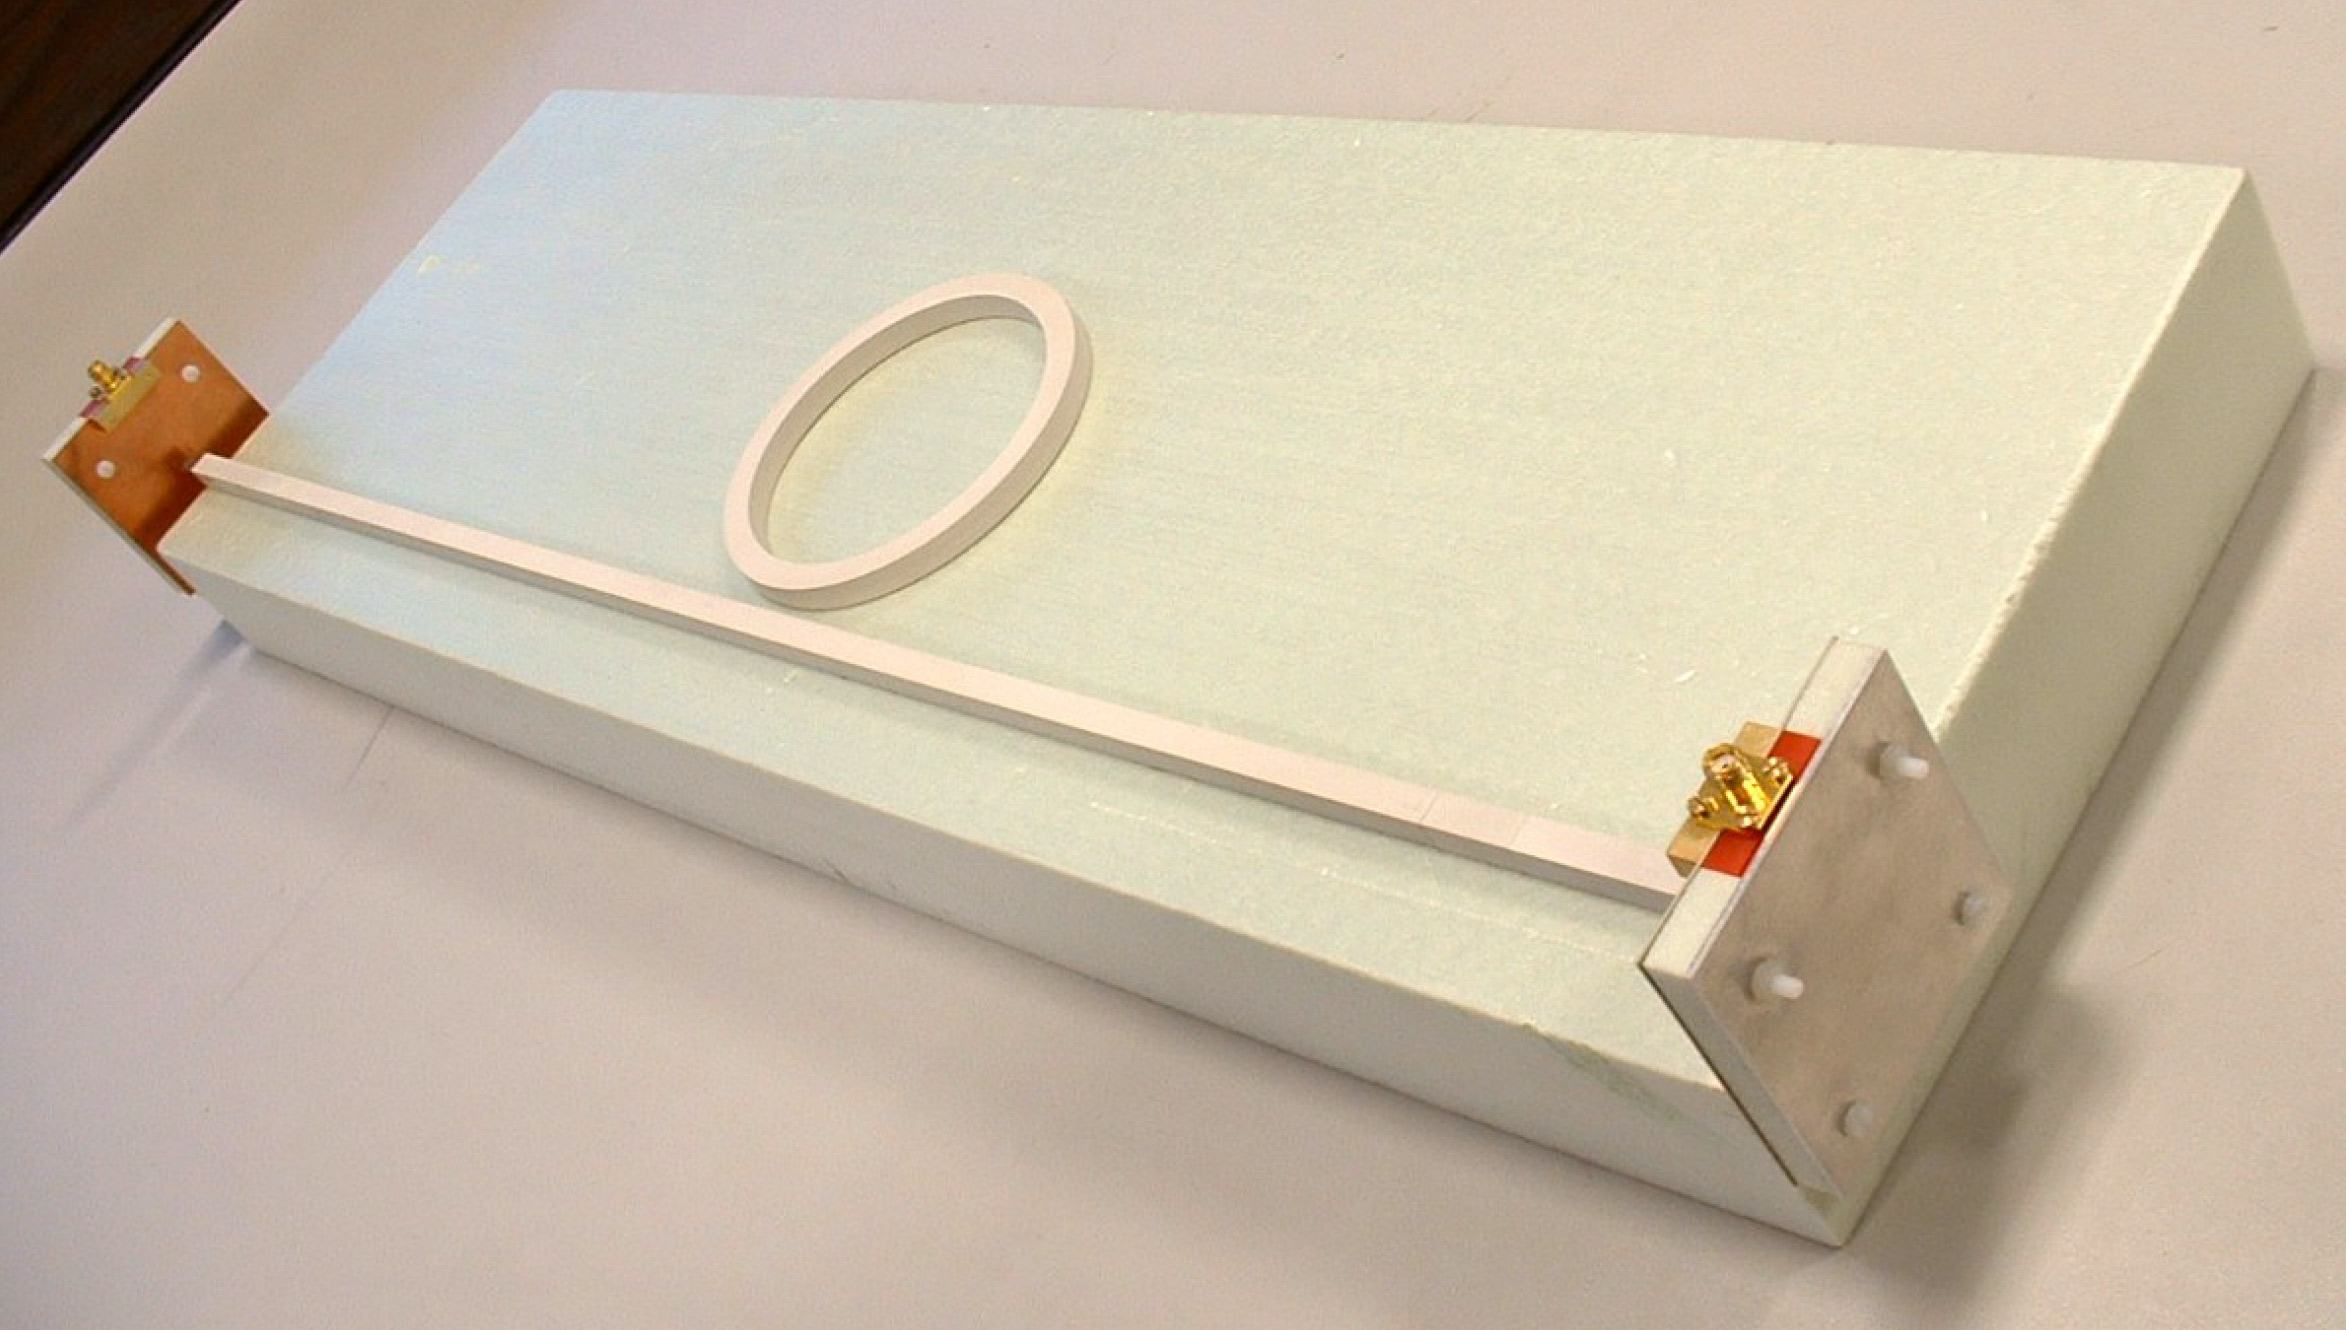
\includegraphics[width=.5\columnwidth]{Grafiken/foto_resonator.jpg}%
\caption{Experimental Setup}%
\label{fig:setup}%
\end{figure}

First a ring with a radius of $r_1$~=~22.6~mm was analyzed. Therefore frequencies between 8 and 10.8~GHz were measuered with 1601 points. The transmission through the setup without any ring resonator was measured and subtracted out with the calibration of the NWA.

The ring was set in direct contact to the line. The transmission changed immediatly. At certain frequencies the transmission breaks in and characteristic dips of the ring resonator can be observed. Figure \ref{fig:01_s21} shows the transmission $|S_{21}|$ through the setup for different distances between the ring and the transmission line.
For lager distance the dips become less deep and the resonance frequency shifts to lower frequencies. The coupling into the ring resonator becomes weaker for higher distances.
 
\begin{figure}%
\centering
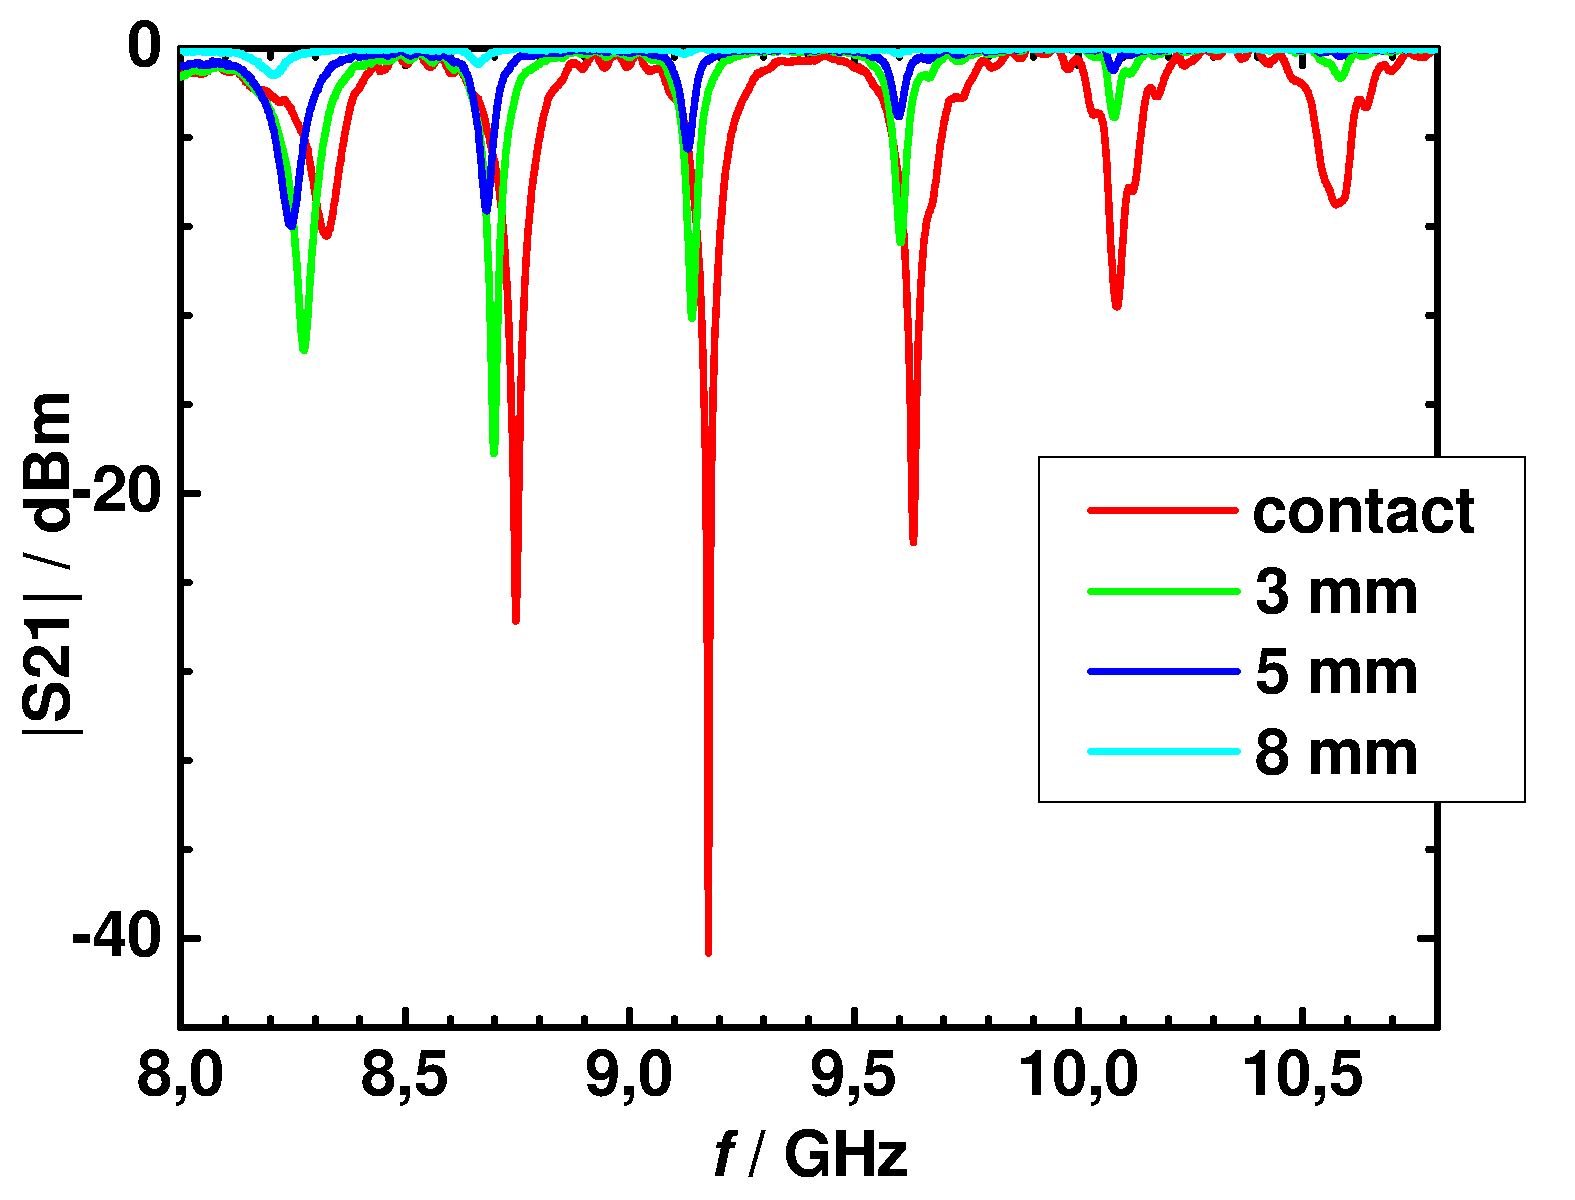
\includegraphics[width=.6\columnwidth]{Grafiken/01_s21.pdf}%
\caption{|$S_{21}$| for different distances between the transmission line and the ring resonator ($r_1$~=~22.6~mm).}%
\label{fig:01_s21}%
\end{figure}

Between a distance of 0~mm and 1~mm the dips become deepest, the transmission gets minimal. In this area there is the case of critical coupling. 

To analyze this the frequency range was changed to 9~GHz~-~9.8~GHz. In this range two dips can be observed. By changing the distance between the ring resonator and the transmission line the minimal transmission at the resonance frequencies was minimized. It was not possible to get both dips below -40~dB. The best result was achieved for a distance of $\sim$0.75~mm. Figure \ref{fig:03_075} shows the transmission for that case.
For this distance $|S_{21}|$(9.16~GHz)~=~-38.3~dB and  $|S_{21}|$(9.62~GHz)~=~-40.3~dB.

$\delta f$ and $\Delta f$ can be extracted from the measurement are given in table \ref{tab:ring_klein}. To read out $\delta f$ the broadness of the dip at |$S_{21}$|~=~-3~dB is measured. 

Using equations \eqref{eq:kappa} and \eqref{eq:alpha} $\kappa$ and $\alpha$ can be calculated.
\begin{equation}
\begin{split}
\kappa(9.16~\mathrm{GHz})=0.44\\
\kappa(9.62~\mathrm{GHz})=0.50
\end{split}
\label{eq:}
\end{equation}
\begin{equation}
\begin{split}
\alpha(9.16~\mathrm{GHz})=4.08~\mathrm{m}^{-1}\\
\alpha(9.62~\mathrm{GHz})=4.85~\mathrm{m}^{-1}
\end{split}
\label{eq:}
\end{equation}

The calculated values for both the resonances are quite different. The transmission above the resonance at 9.62~GHz is uneven. Because of this maybe the $\delta f$ is not good enough to measure. 

\begin{figure}%
\centering
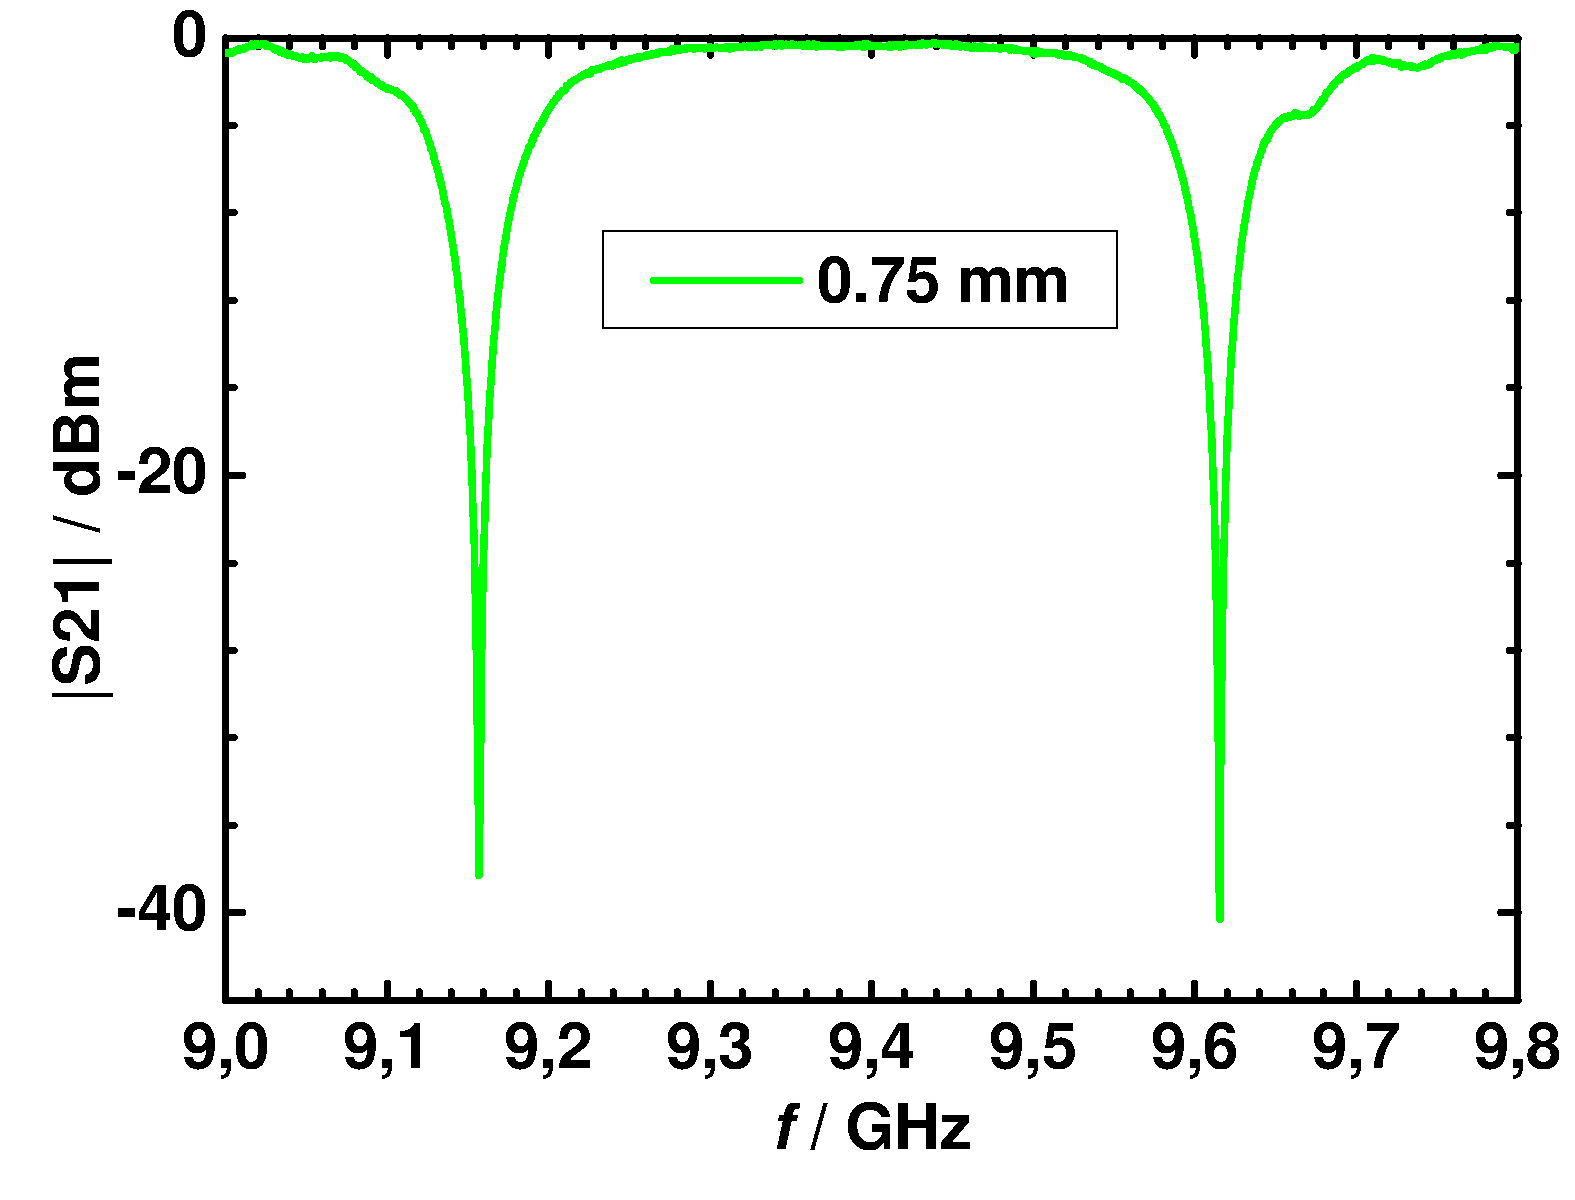
\includegraphics[width=.6\columnwidth]{Grafiken/03_075.pdf}%
\caption{Transmission near the case of critical coupling for a small ring ($r_1$~=~22.6~mm)}%
\label{fig:03_075}%
\end{figure}

Secondly a larger ring with a radius of $r_2$~=~45.1~mm was examined. Comparing the small and the large ring (cf. fig. \ref{fig:04_vergleich}) the large ring shows in the same frequency range twice as much resonances compared to the small ring. This agrees with equation \eqref{eq:abstand} since the  radius of the resonator and therefore length of the resonator has doubled thus the distance between two resonances $\Delta f$ halves.
\begin{figure}%
\centering
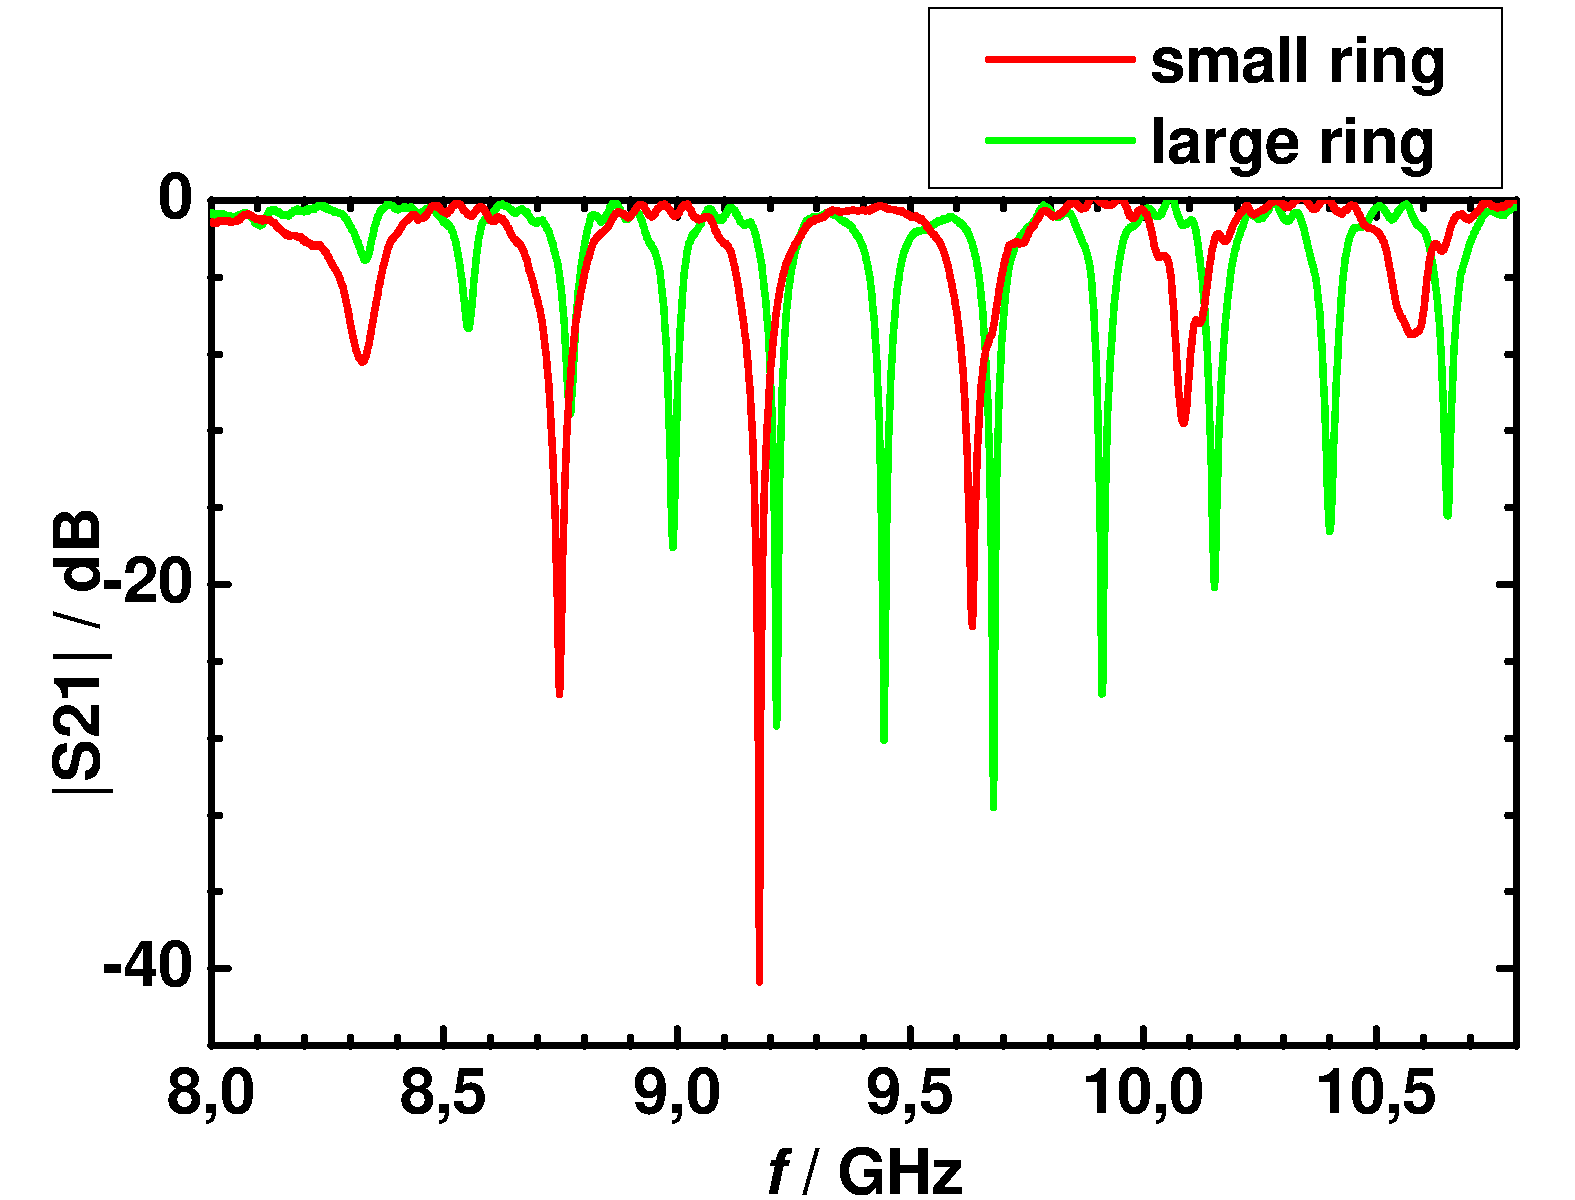
\includegraphics[width=.6\columnwidth]{Grafiken/04_vergleich.pdf}%
\caption{Transmission of the small ring ($r_1$~=~22.6~mm) resonator and a large ring ($r_2$~=~25.1~mm)  resonator.}%
\label{fig:04_vergleich}%
\end{figure}

\begin{figure}%
\centering
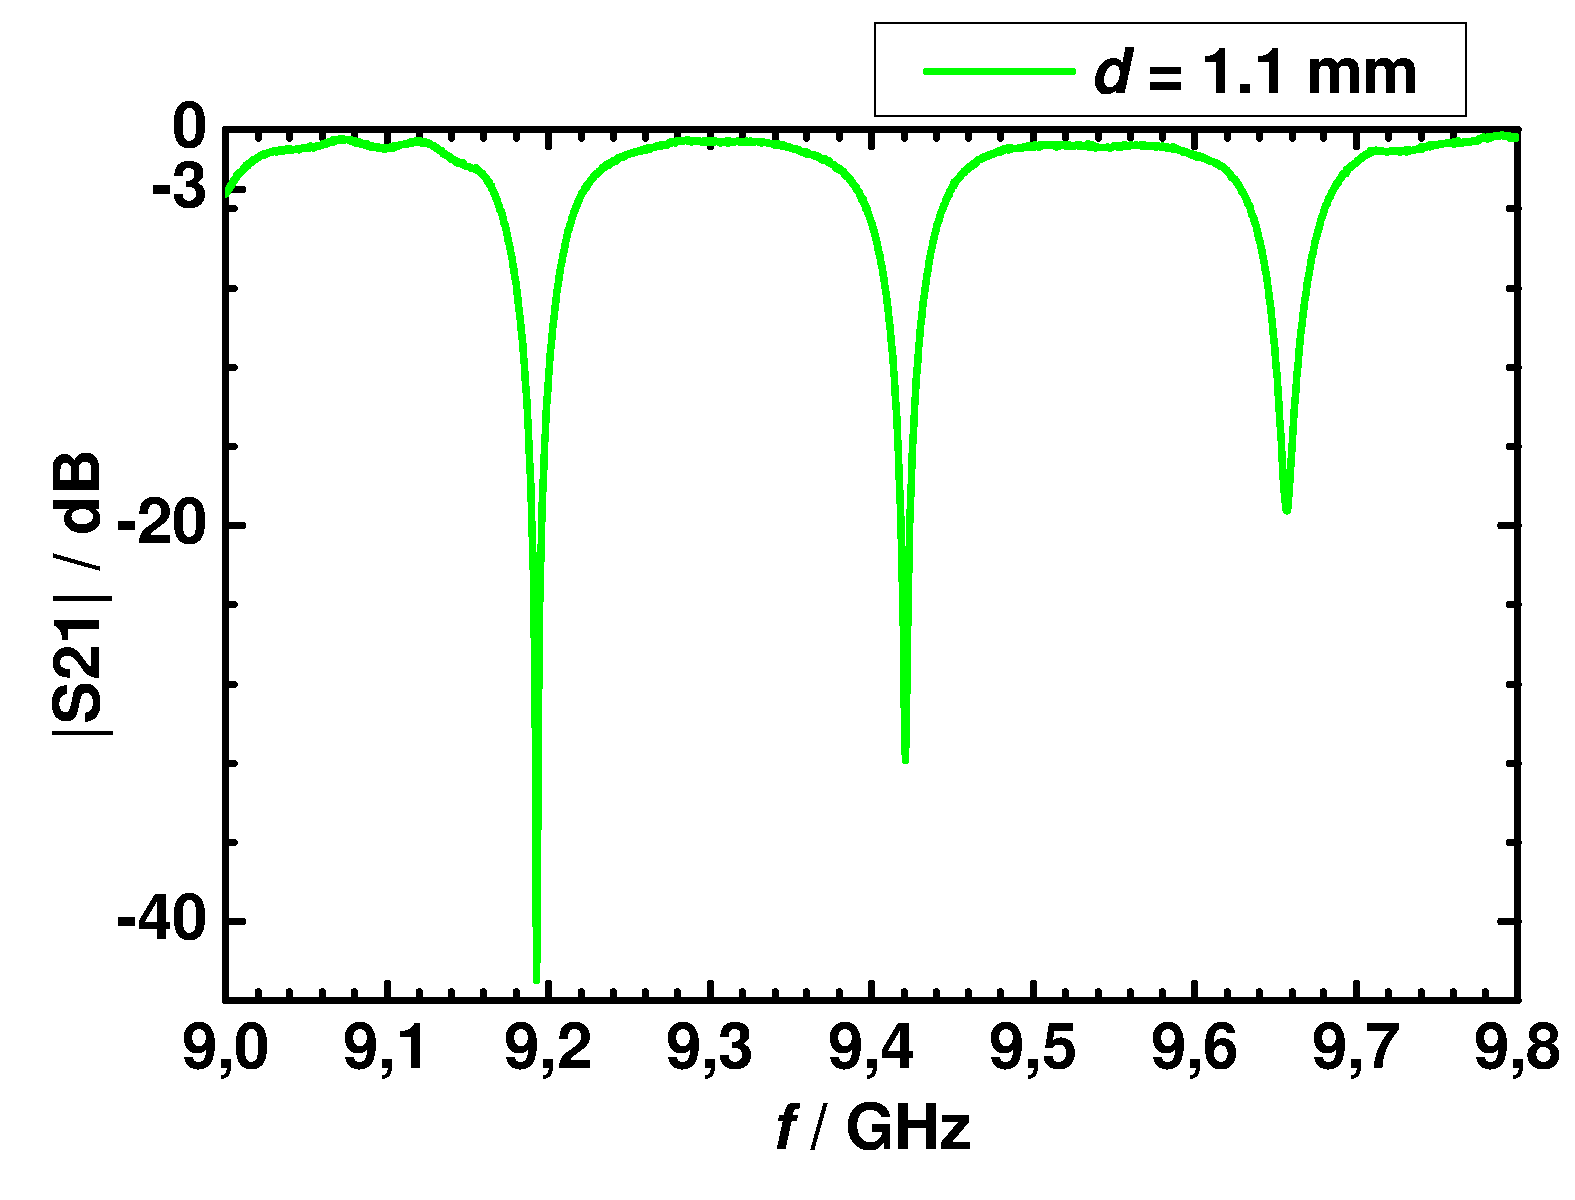
\includegraphics[width=.6\columnwidth]{Grafiken/05_11.pdf}%
\caption{Transmission near the case of critical coupling for a large ring ($r_2$~=~45.1~mm)}%
\label{fig:05_11}%
\end{figure}
Again the distance between the ring and the transmission line was varied to get the lowest transmission at the resonances. \\The best result was achieved at a distance of $\sim$1.1~mm. Here the transmission of at least one resonance is below \mbox{-40~dB}.
The measured transmissions at $d \approx 1.1$~mm are |$S_{21}$|(9.19~GHz)~=~\mbox{-43.0~dB}, |$S_{21}$|(9.42~GHz)~=~\mbox{-32.9~dB} and |$S_{21}$|(9.66~GHz)~=~-19.3~dB.

Assuming that this is the case of critical coupling the coupling coefficient $\kappa$ and the attenuation $\alpha$ can be calculated as before. The values used to calculate are given in table \ref{tab:ring_gross}.
\begin{equation}
\begin{split}
\kappa(9.19~\mathrm{GHz})=0.53\\
\kappa(9.42~\mathrm{GHz})=0.57\\
\kappa(9.66~\mathrm{GHz})=0.54\\
\end{split}
\label{eq:}
\end{equation}
\begin{equation}
\begin{split}
\alpha(9.19~\mathrm{GHz})=2.68~\mathrm{m}^{-1}\\
\alpha(9.42~\mathrm{GHz})=3.00~\mathrm{m}^{-1}\\
\alpha(9.66~\mathrm{GHz})=2.72~\mathrm{m}^{-1}
\end{split}
\label{eq:}
\end{equation}

Comparing the data measured and calculated for the small and the large resonator shows that the attenuation of the larger ring is higher than the attenuation of the small ring. This could be explained by the smaller bending radius of the small ring. 
But since the lenght of the waveguide of the large ring is larger the total losses over the length are higher then the losses in the small resonator. Thus the condition for critical coupling (cf. \eqref{eq:crti}) leads to a larger coupling coefficient $\kappa$ at critical coupling for the large resonator.

\begin{table}%
\centering
\caption{Ring resonator ($r_1$~=~22.6~mm) at critical coupling ($d \approx 0.75$~mm). Transmission properties.}
\begin{tabular}{cccccc}
\toprule
$f\i{res}$	& $\delta f$	& $\Delta f$ & $F$ & $\kappa$ & $\alpha$\\
\midrule
9.16 GHz	& 0,086~GHz	& 0.46~GHz	&	5.35&	0.44 & 4.08~m$^{-1}$\\
9.62 GHz	& 0,103~GHz	& 0.46~GHz	&	4.47	&	0.50 & 4.85~m$^{-1}$\\
\bottomrule 
\end{tabular}
\label{tab:ring_klein}
\end{table}

\begin{table}%
\centering
\caption{Ring resonator ($r_2$~=~45.1~mm) at critical coupling ($d \approx 1.1$~mm). Transmission properties.}
\begin{tabular}{cccccc}
\toprule
$f\i{res}$	& $\delta f$	& $\Delta f$ & $F$ & $\kappa$ & $\alpha$\\
\midrule
9.19 GHz	& 0.057~GHz	& 0.23~GHz	& 4,04	& 0.53	& 2.68~m$^{-1}$ \\
9.42~GHz	&	0.064~GHz	&	0.23~GHz	& 3,59	& 0.57	&	3.00~m$^{-1}$\\
9.66 GHz	& 0,058~GHz	& 0.23~GHz	&	3,97	&	0.54	& 2.72~m$^{-1}$ \\
\bottomrule 
\end{tabular}
\label{tab:ring_gross}
\end{table}

\newpage
The next task was to analyze the group delay change when varying the distance of the ring. Therefore the format of the NWA display was changed to $gruop~delay$. The frequency range was defined as 8.55-9.85~GHz.

\begin{figure}[t]%
\centering
%\begin{adjustwidth}{0cm}{0cm}
%	\subfloat[contact]{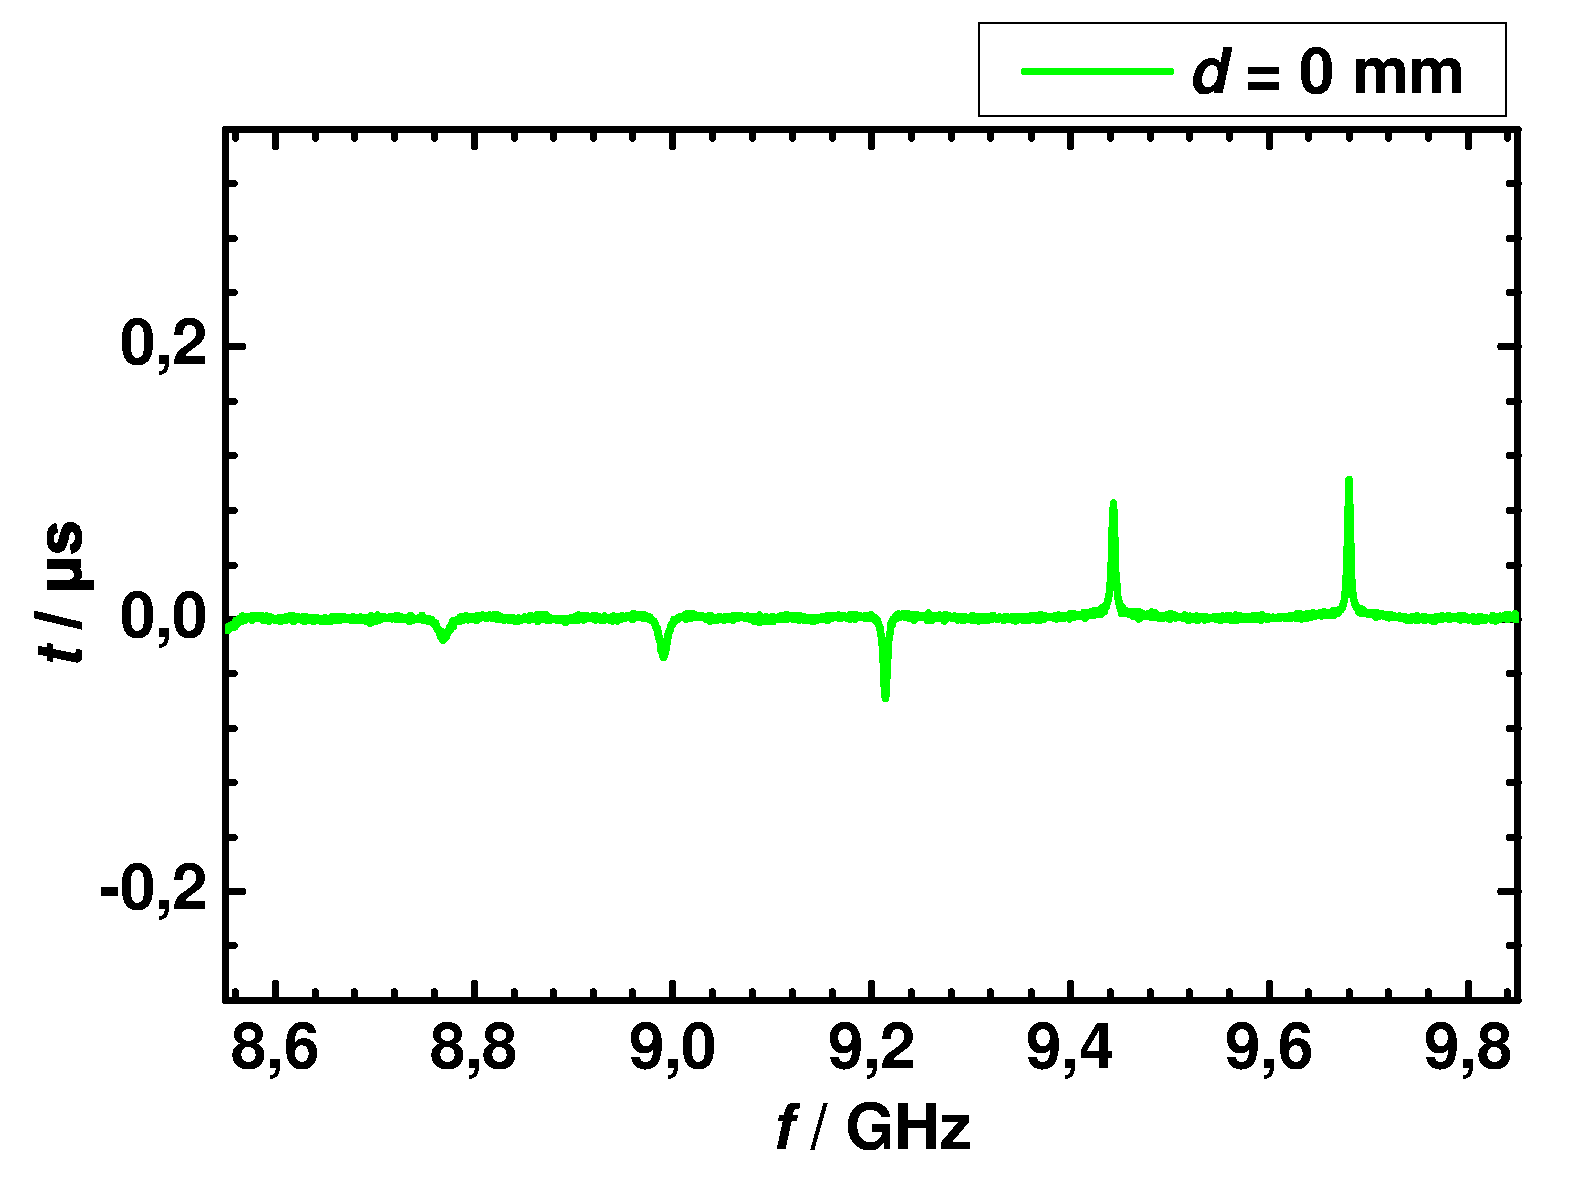
\includegraphics[totalheight=6 cm]{Grafiken/06_0.pdf}\label{fig:06_0}}
	\subfloat[$d = 0.7$~mm]{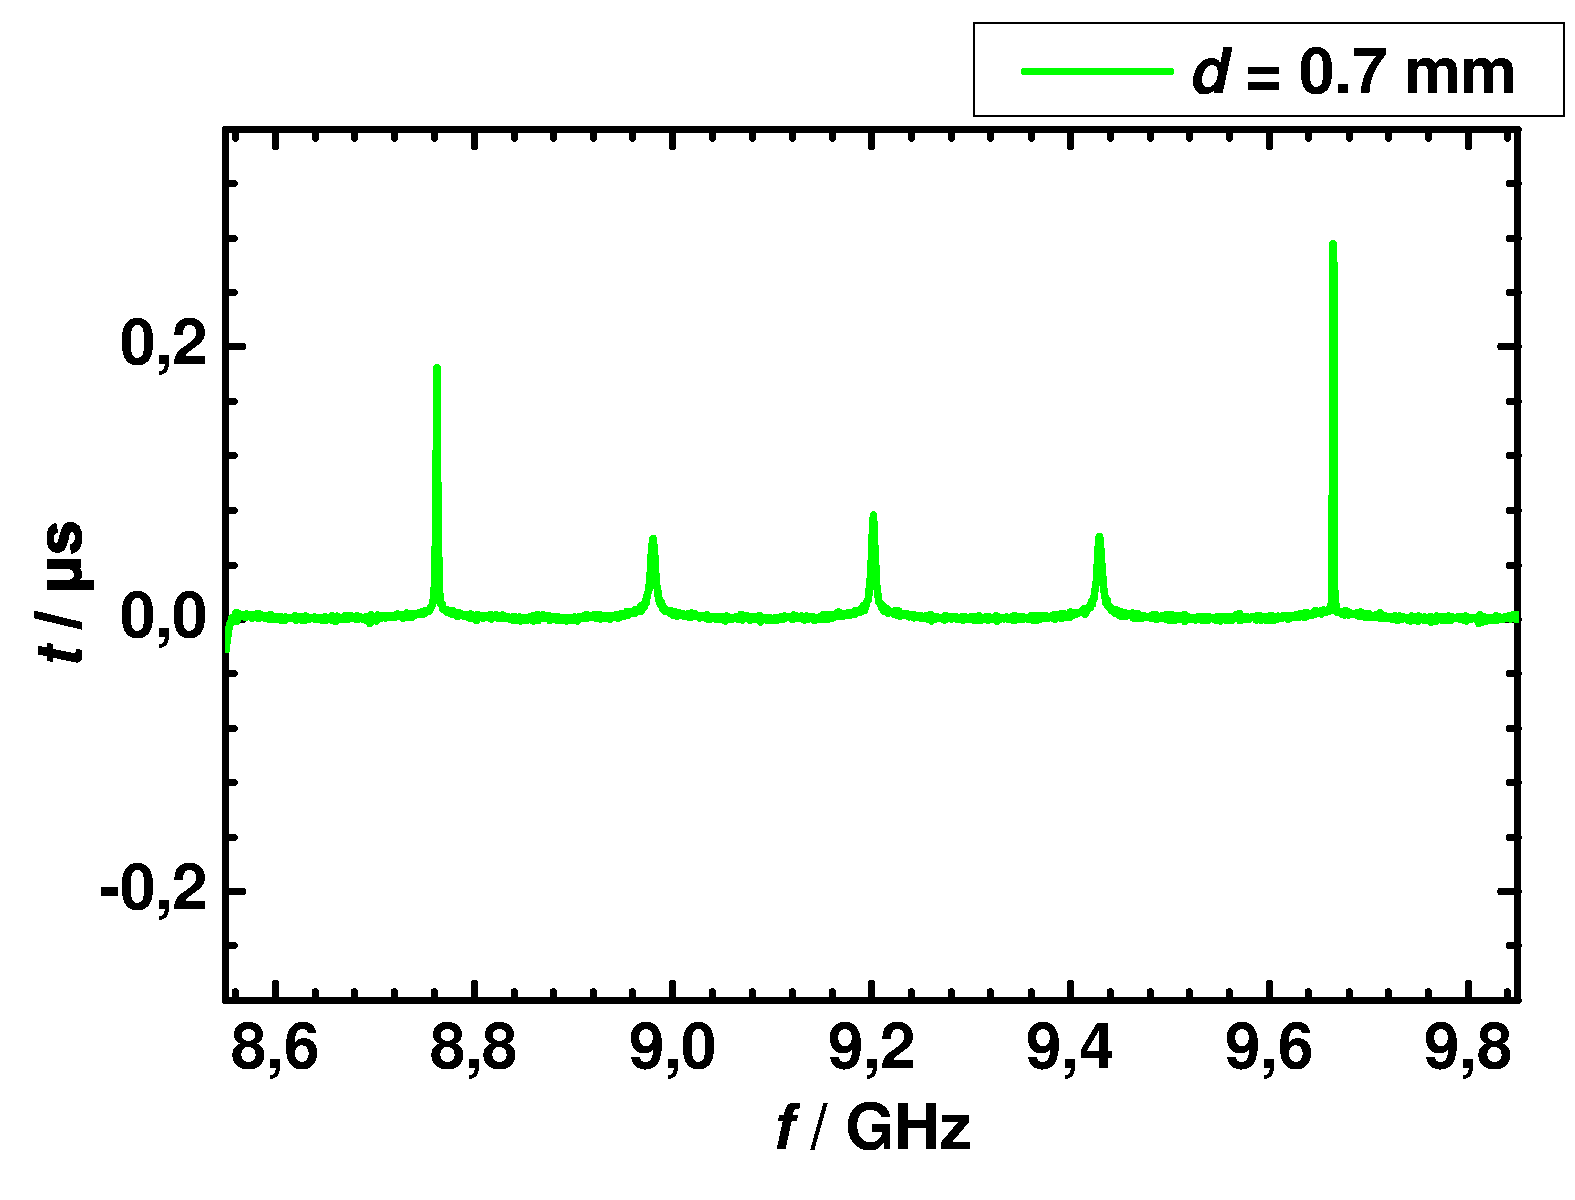
\includegraphics[totalheight=6 cm]{Grafiken/06_07.pdf} \label{fig:06_07}}
		\subfloat[$d = 1.2$~mm]{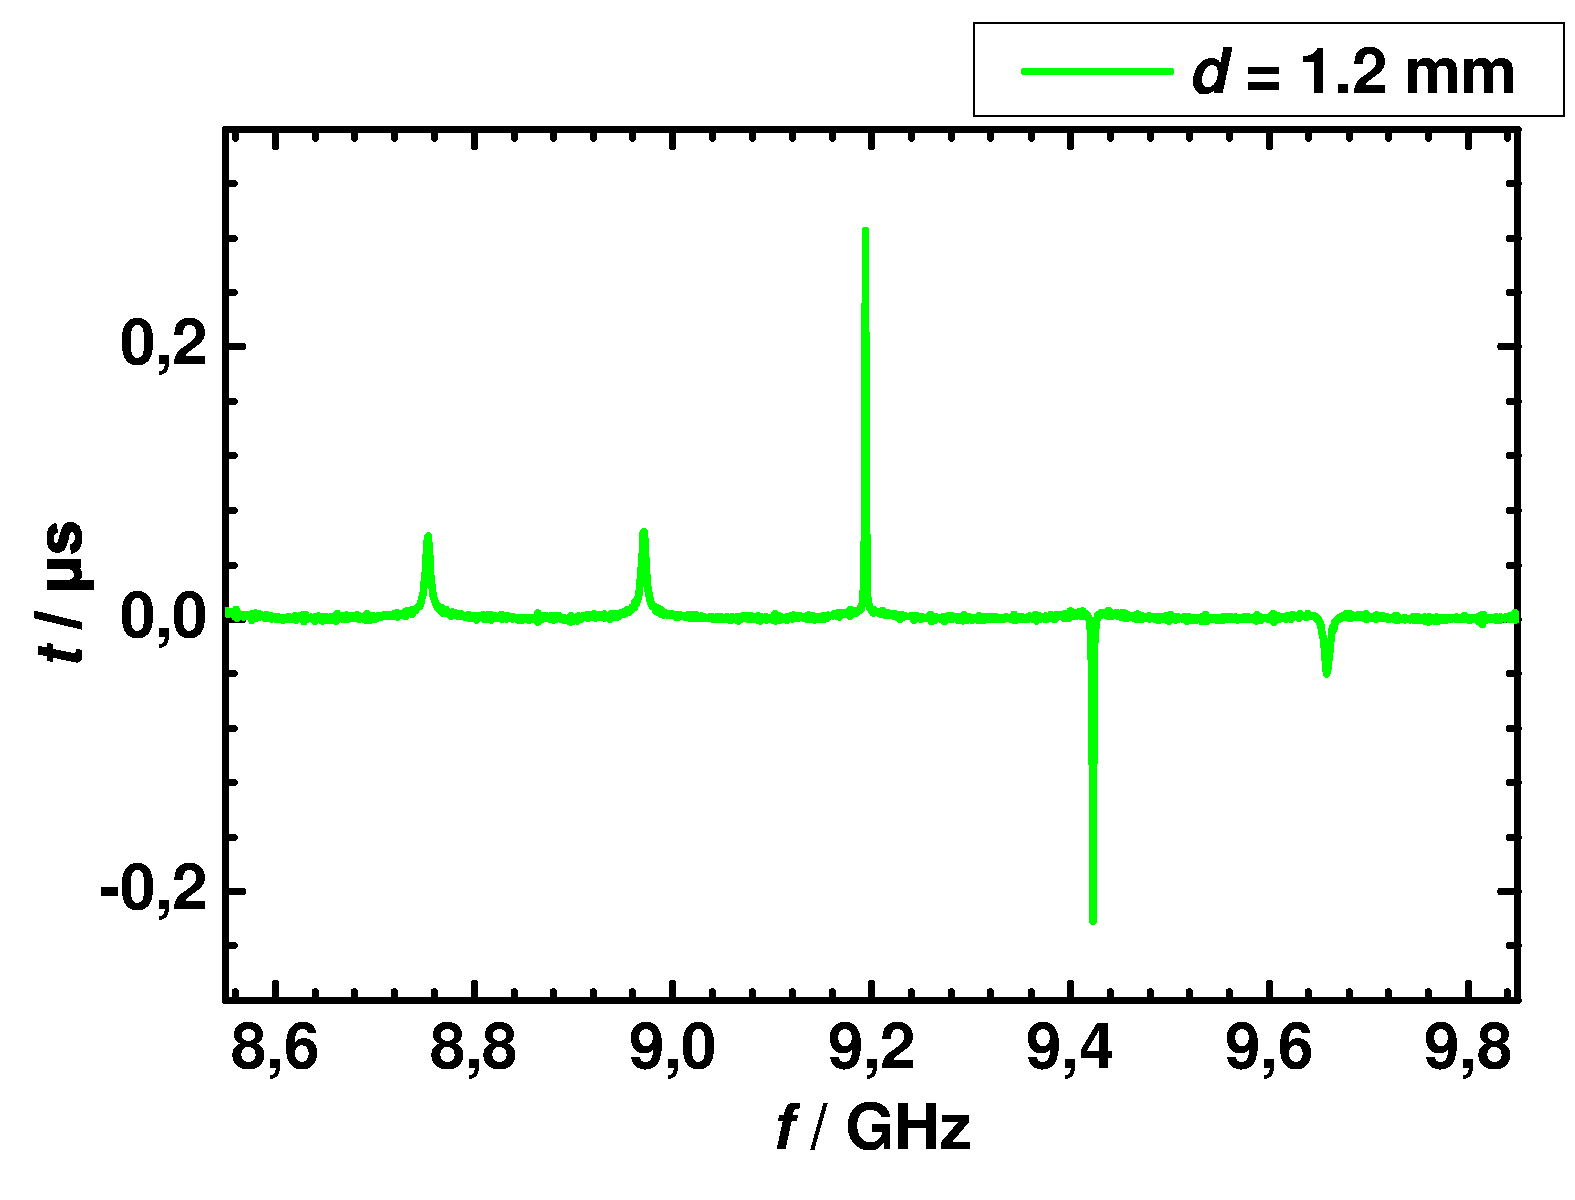
\includegraphics[totalheight=6 cm]{Grafiken/06_12.pdf}\label{fig:06_12}}\\
	\subfloat[$d = 2.2$~mm]{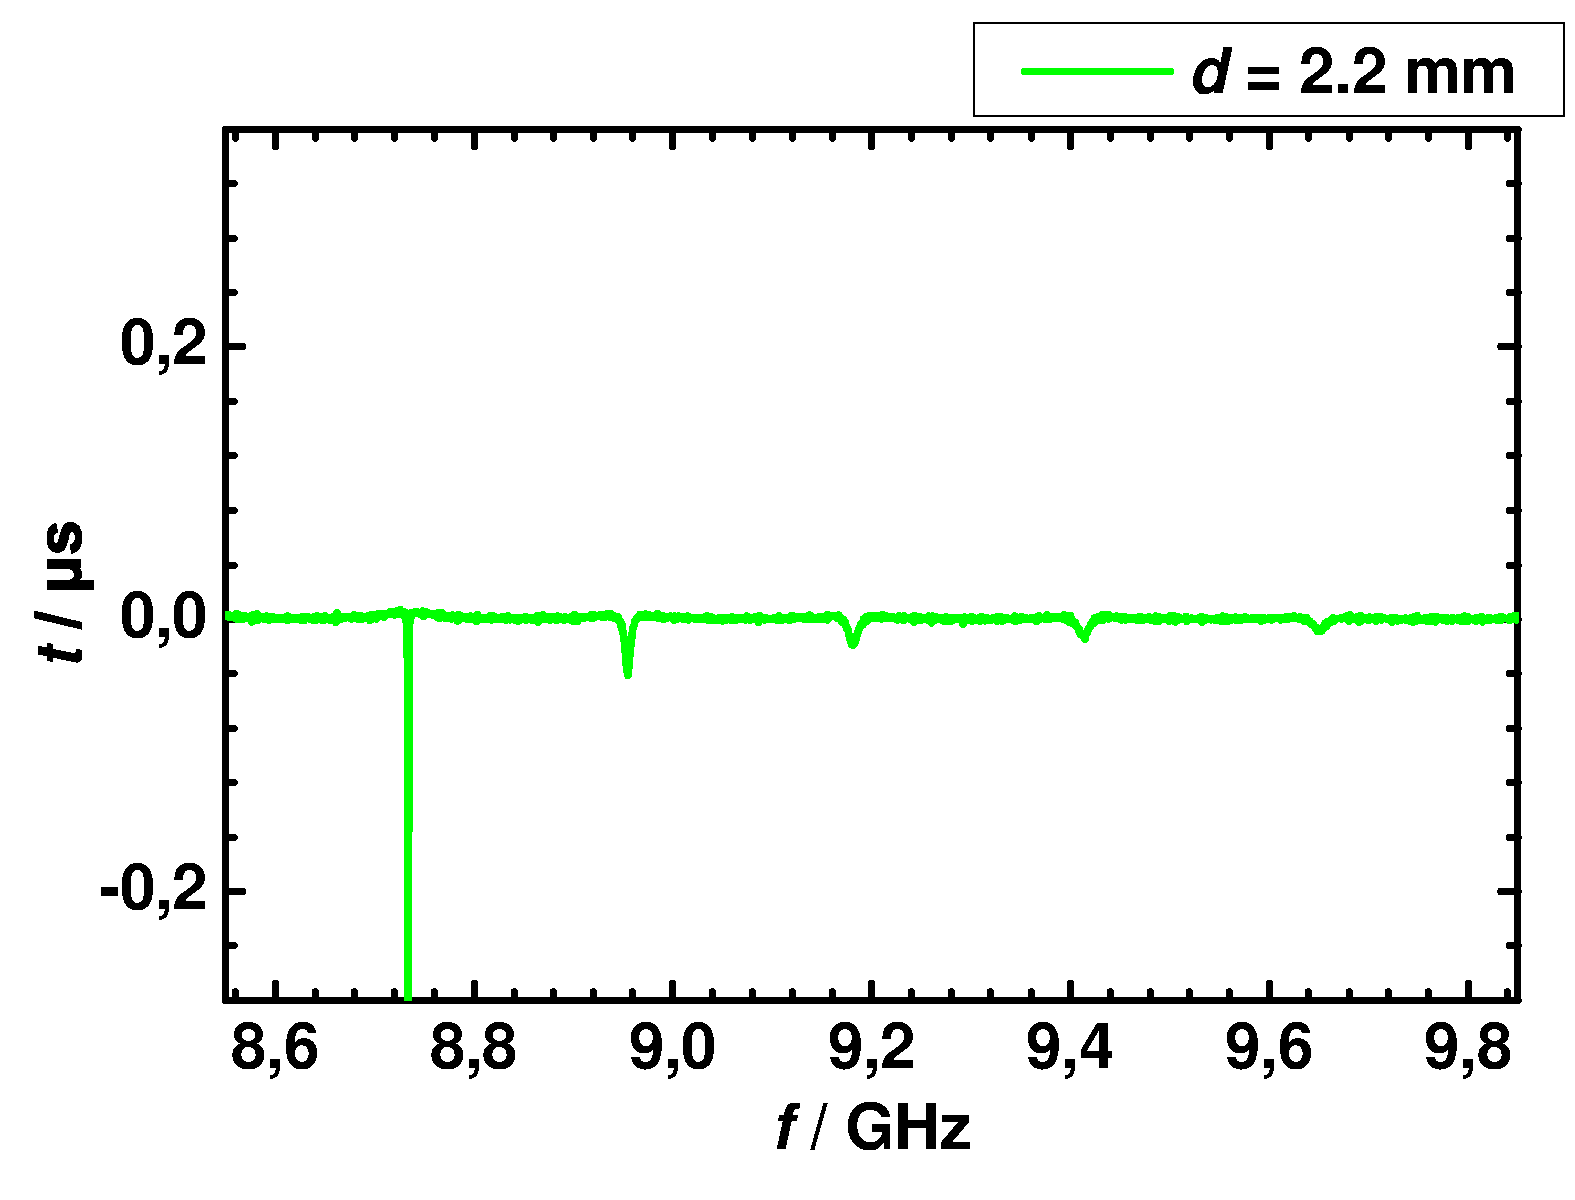
\includegraphics[totalheight=6 cm]{Grafiken/06_22.pdf} \label{fig:06_22}}
\caption{Group delay for different distances of the ring.}%
\label{fig:06}%
\end{figure}
When moving the ring slowly away from the transmission line one can observe a change in group delay. At first, near the transmission line the transmission at the resonances has a positive group delay (cf. fig. \ref{fig:06_07}). This is the case of overcritical coupling. Here the losses in the ring are higher than the coupling losses and the signal gets delayed. Moving the ring away at one specific point the group delay changes from positive to negative \ref{fig:06_12}). This behavior can be observed at a distance of $\sim$1.2~mm. This point can be assumed as the point of critical coupling, where the coupling losses are equal to the losses in the resonator. In theory at critical coupling the group delay should be zero. Since this is a real and no ideal resonator this can't be observed.
Moving the ring further away the group delay gets negative. This is the case of undercritical coupling, where the coupling losses exceed the resonator losses. 

Last both rings were coupled to the straight waveguide. The distance between both rings were large, that no field could cuople from one ring in the other. Figure \ref{fig:07} shows the transmission for this setup for different distances from the straight line. The resonances of both rings are visible. Because the large ring shows twice as much resonances as the small ring only every second resonance shows two dips. By changing the distance between the rings and the straight line the position of the resonances can be adjusted as well as the depth of one dip.

This shows that using different ring resonators in series filters can be realized (cf. \ref{design}).


\begin{figure}%
\centering
	\subfloat[]{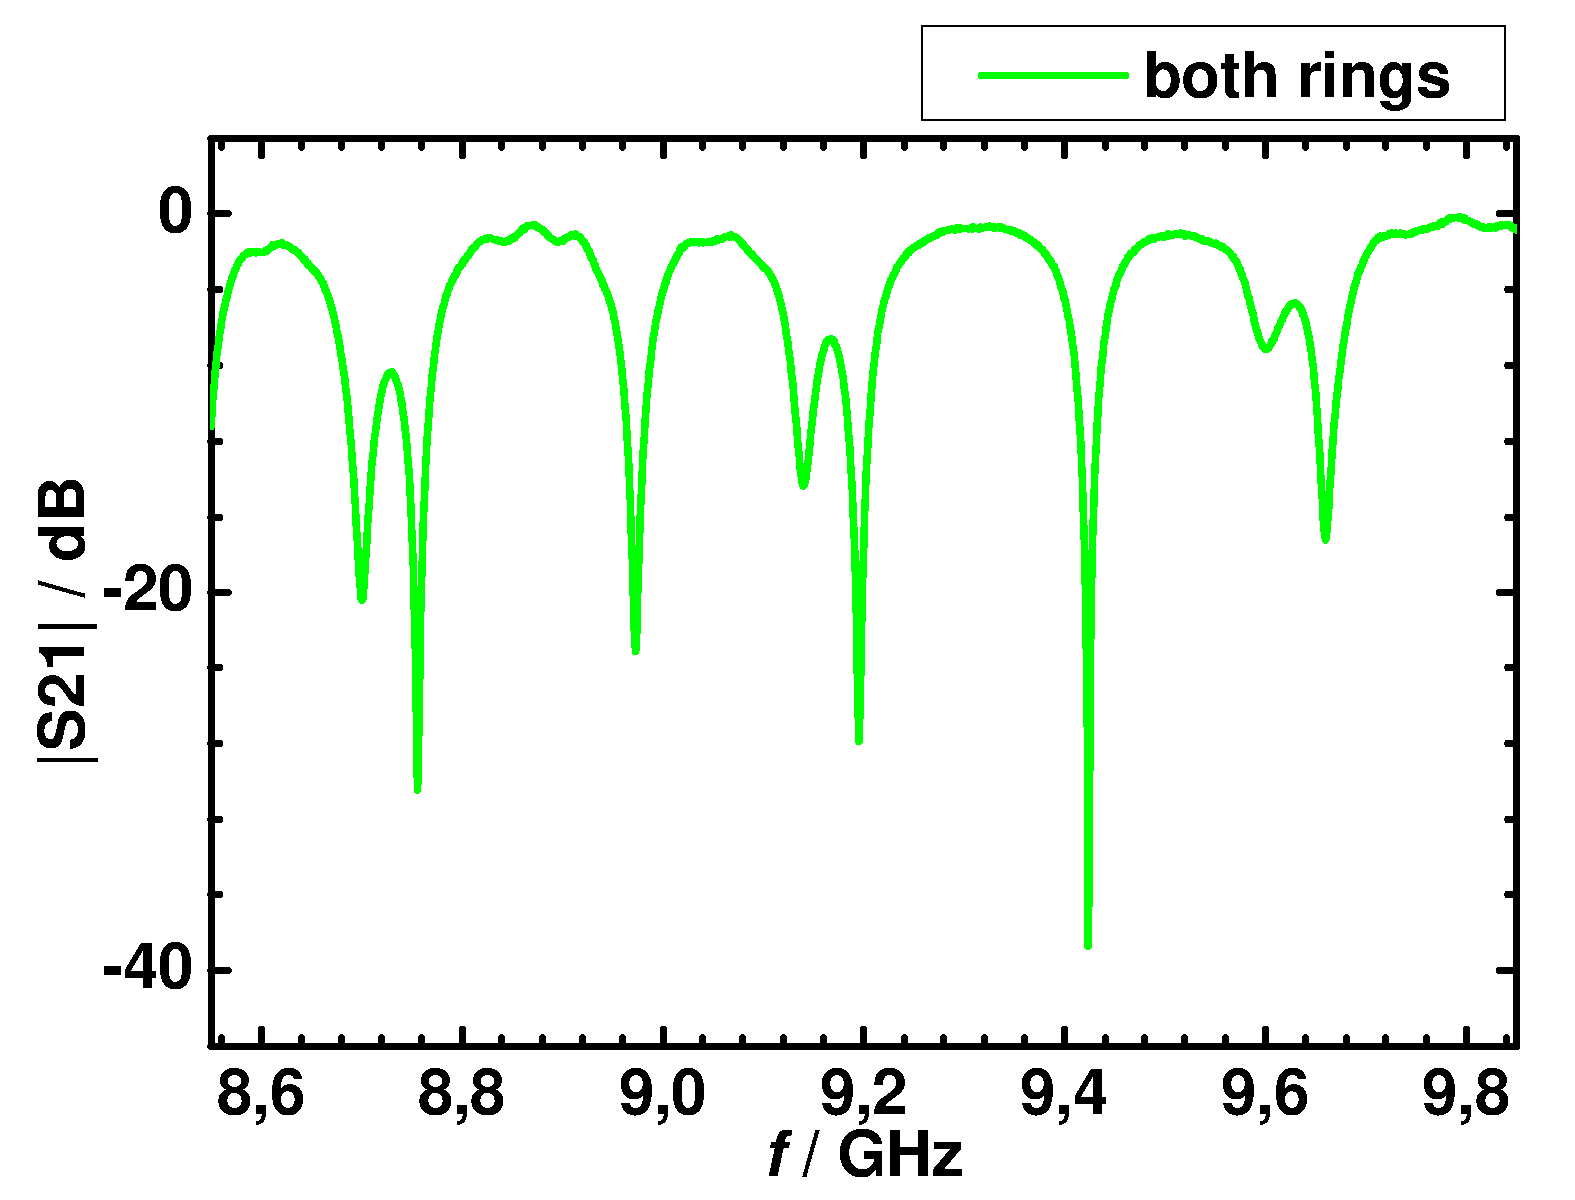
\includegraphics[totalheight=6 cm]{Grafiken/07_both.pdf} \label{fig:07_1}}
		\subfloat[]{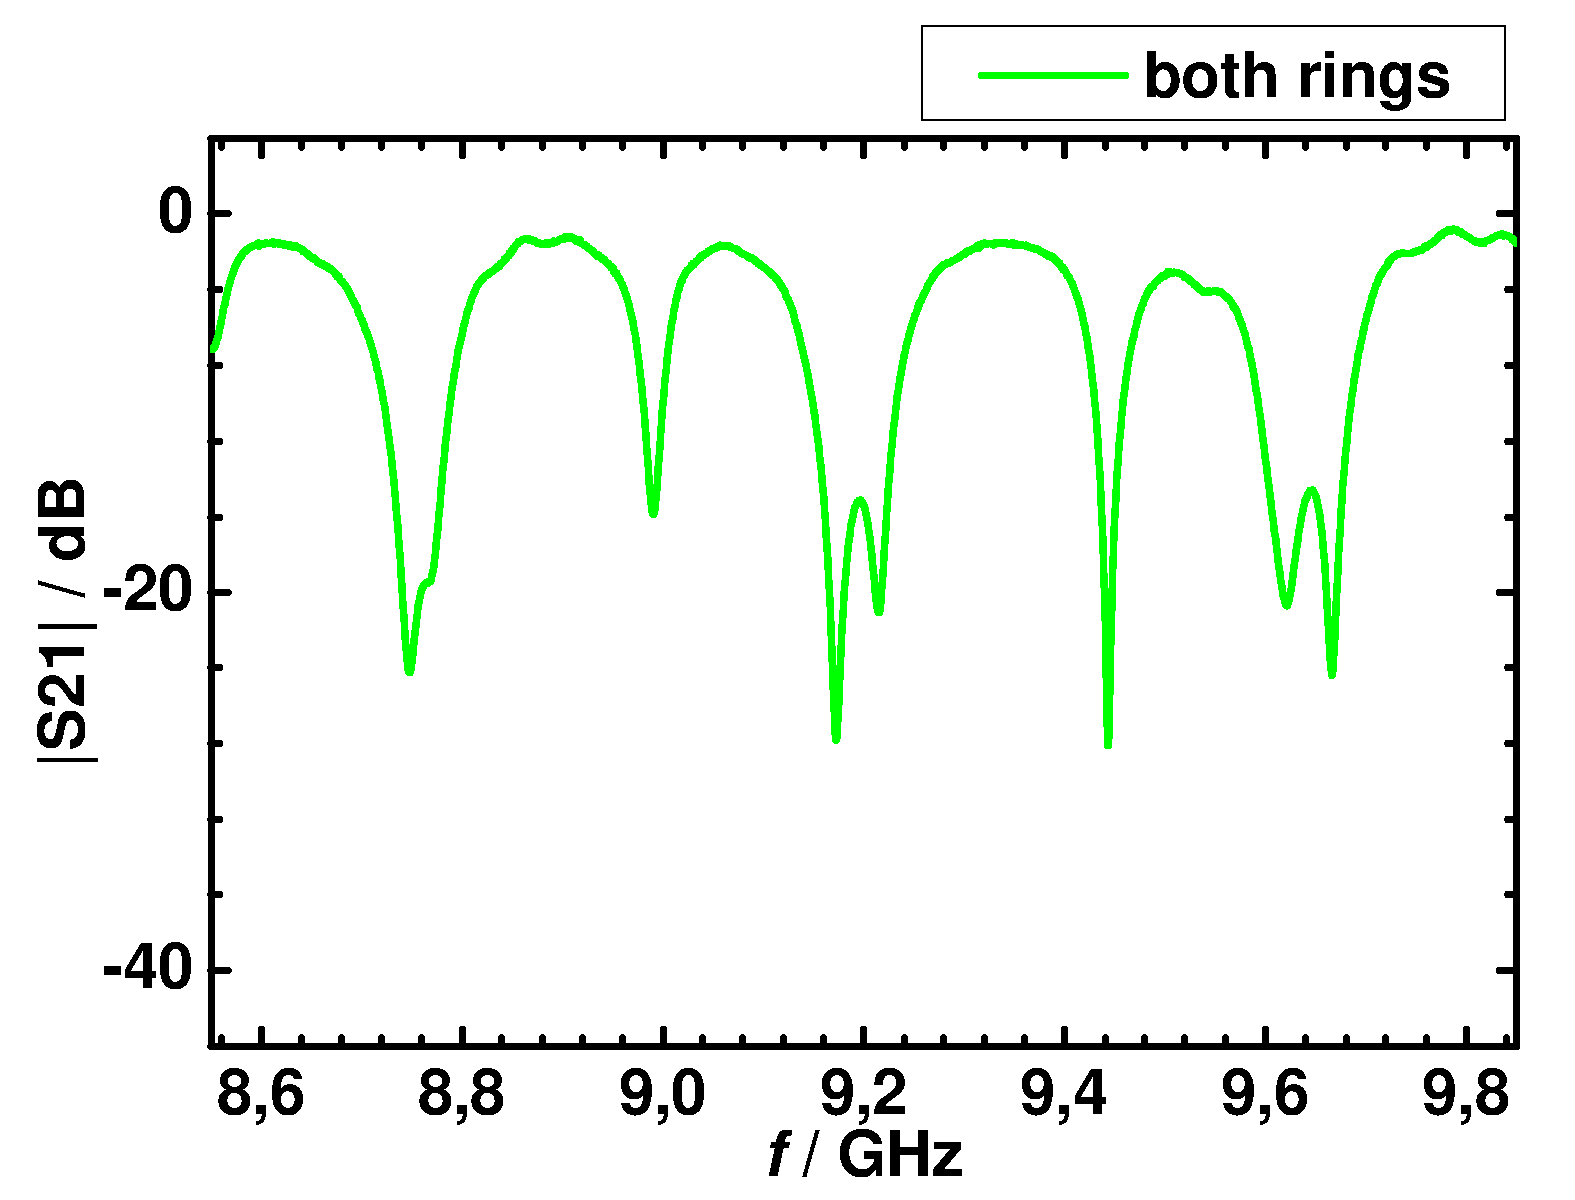
\includegraphics[totalheight=6 cm]{Grafiken/07_both2.pdf}\label{fig:06_2}}
\caption{Transmission with both rings near the straight waveguide.}%
\label{fig:07}%
\end{figure}

\chapter{Simulation}
\begin{figure}[ht]
\centering
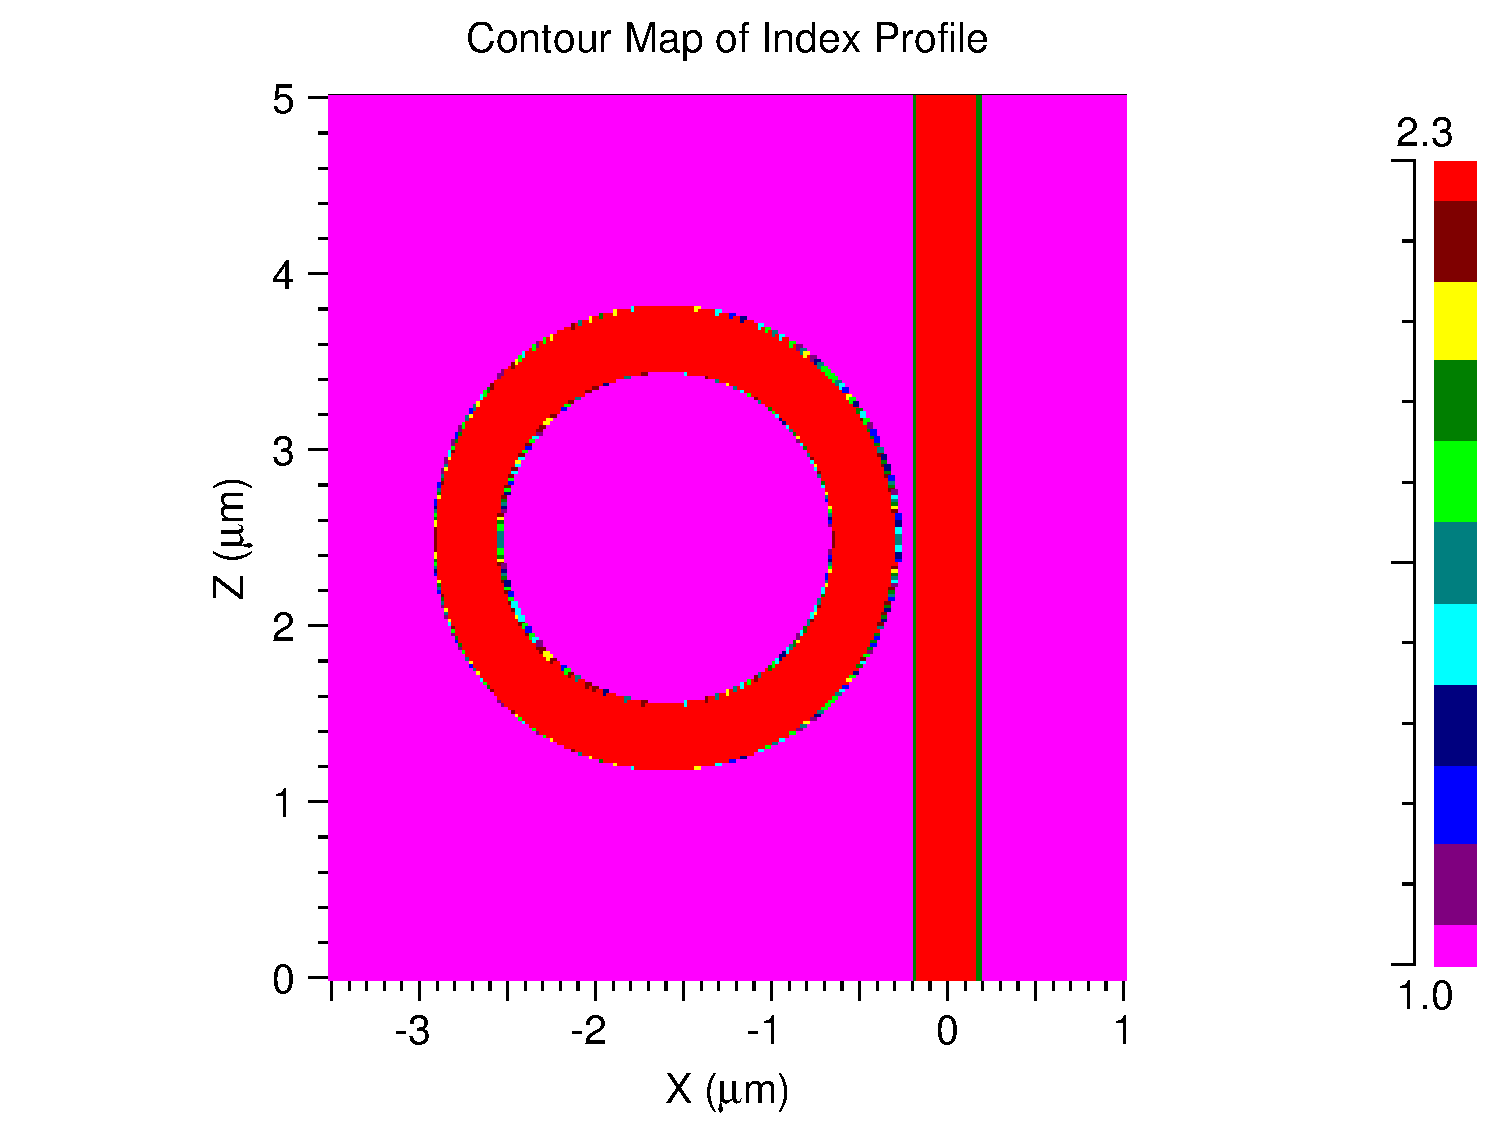
\includegraphics[width=.6\columnwidth]{Grafiken/11_index_profile.pdf}%
\caption{Index profile of the simulated waveguide structure}%
\label{fig:index_profile1}%
\end{figure}

In the next step a simulation with the program RSoft was performed. To reduce the computation time the 3D-structure was reduced to a 2D-structure using the effective index method. The simulation was performed in the optical frequency domain around 200~THz, so the dimensions of the waveguides had to be reduced by a factor of 20000. 

The strip waveguide with a length $l=5~\upmu$m was drawn in z-direction. For drawing the resonator rings two concentric cylinders with different diameters were created and subtracted from each other. The resulting index profile of the structure is shown in figure \ref{fig:index_profile1}.
% 
% \begin{figure}[ht]
% \centering
% 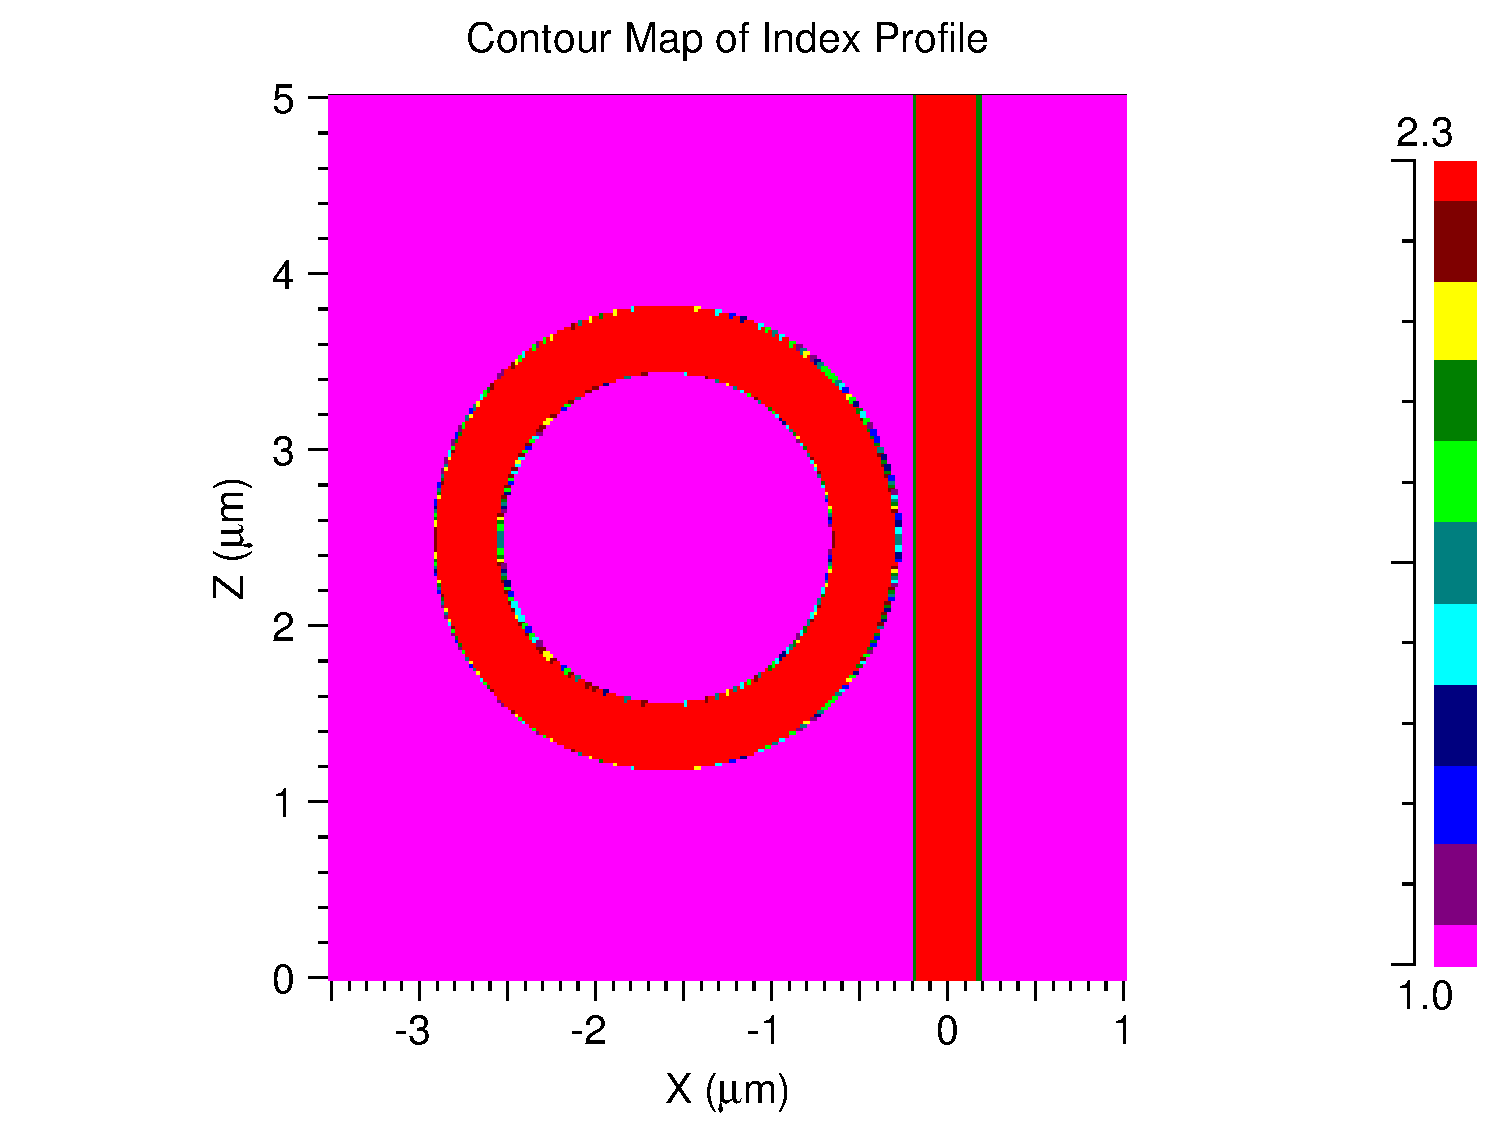
\includegraphics[width=.6\columnwidth]{Grafiken/11_index_profile.pdf}%
% \caption{Index profile of the simulated waveguide structure}%
% \label{fig:index_profile1}%
% \end{figure}



In the first simulation the waveguide is exited by a pulse. The pulse propagates through the waveguide structure. At the output the impulse response of the transimission can be recorded. By performing a fourier transform the frequency behavior of the system can be examined. Figure \ref{fig:2_TE_FFT} shows the fourier transform of the input signal (red) and the output signal (green). Deviding the input signal through the output signal results in the transmission $\left|S_{21}\right|$ in dependency of the frequency, like examined in the preceeding experiment (cf. \ref{ch:part1}). Therefore the resonance frequencies can be read from the dips in figure \ref{fig:2_TE_FFT}. The free spectral range (FSR) can be determined by subtracting to neighbouring resonance frequencies. With the dips at  $195$~THz and $211,5$~THz the FSR results to $FSR = 16.5$~THz.


\begin{figure}
\centering
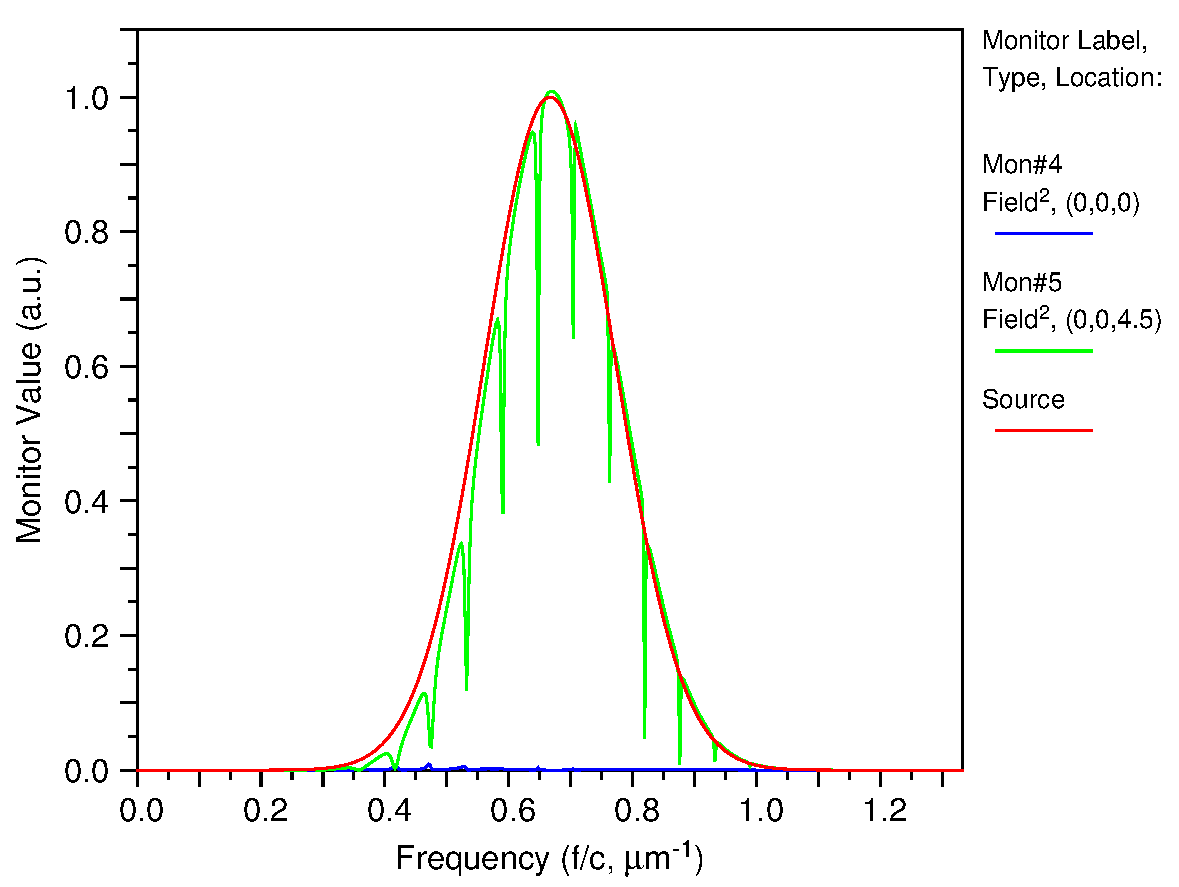
\includegraphics[width=.6\columnwidth]{Grafiken/12_TE_FFT.pdf}%
\caption{FFT of the input signal (red) and the output signal (green)}%
\label{fig:2_TE_FFT}%
\end{figure}



\newpage
In the next simulation the two resonance frequencies at $195$~THz and $211,5$~THz and the intermediate frequency at 202.7~THz is examined. Now the waveguide is exited by a current wave (CW) and the spatial field distribution and the the field at the output in dependence of time is examined (cf. figures \ref{fig:13_54}, \ref{fig:13_48} and \ref{fig:13_42}).

For the resonance frequency of 195~THz the spatial field distribution is shown in figure \ref{fig:3_1_54_aufsicht}. The CW couples in the resonator continously. At the beginnig the resonator doesnt guide a wave and thus nothing couples out. Therefore the wave transmitted to the output is only dependent of the coupling factor $\kappa$. After one circulation a part of the light couples out and interferres destructively with the incident wave. Thus the signal decreases. Every further time the wave circulates the wave couples out too. At some time more waves are coupled out of the resonator, than are coupled in. Thus the output signal increases. This behavior can be seen in figure \ref{fig:3_1_54_field}. There are 4 wavelenght fitting in the resonator until the outcoupling gets larger than the transmission to the output. 

For the frequency of $211.5$~THz the field distribution is shown in figure \ref{fig:3_1_48_aufsicht}. The field in the resonator is much lower than at the resonance frequencies because the wave doesn't fit in the resonator. At the beginning the wave couples in the waveguide like at the resonance frequencies. After one circulation light a part of the light couples out and interferres constructively with the incident wave at the output. Thus the transmission is greater than 1. But the circulating wave interferres destructively with the wave coupled in. Thus the intensity of the circulating wave decreases and the transmission reaches value arround 1 after infinite time. This behavior can be examined in figure \ref{fig:3_1_48_field}.
\newpage
For the resonance frequency of 211,5~THz the behavior is the same as at the resonance frequency of 195~THz. Only there are more wavelength fitting in the resonator, because of the shorter wavelength. Thus there are 7 wavelength fitting in the resonator. This behavior can be examined in figure \ref{fig:3_1_42_field}.

 
\begin{figure}%
\centering
	\subfloat[]{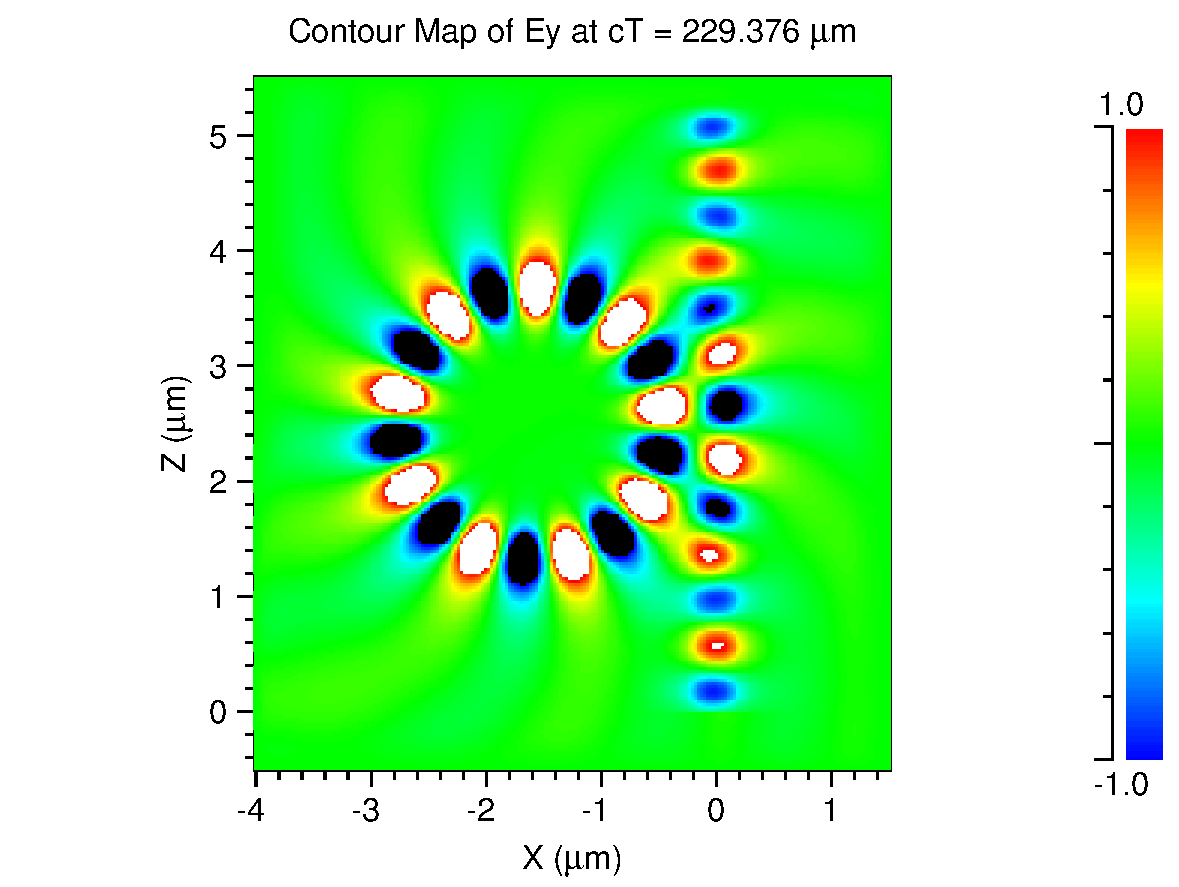
\includegraphics[totalheight=5 cm]{Grafiken/13_54_aufsicht.pdf}\label{fig:3_1_54_aufsicht}}
	\subfloat[]{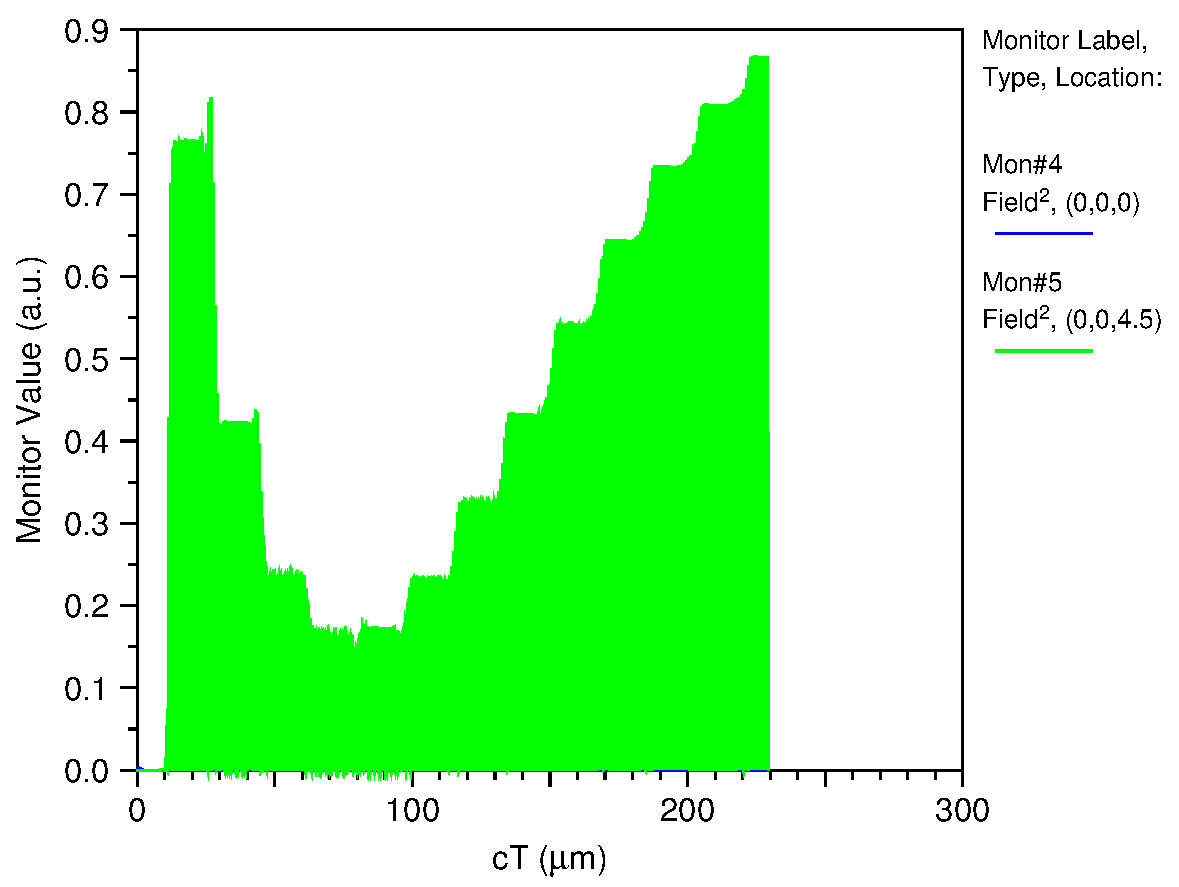
\includegraphics[totalheight=5 cm]{Grafiken/13_54_field.pdf} \label{fig:3_1_54_field}}\\%
\caption{Spatial Field Distribution \textbf{(a)} and Field at the Output \textbf{(b)} for a frequency of 195~THz}%
\label{fig:13_54}%
\end{figure}

\begin{figure}%
\centering
	\subfloat[]{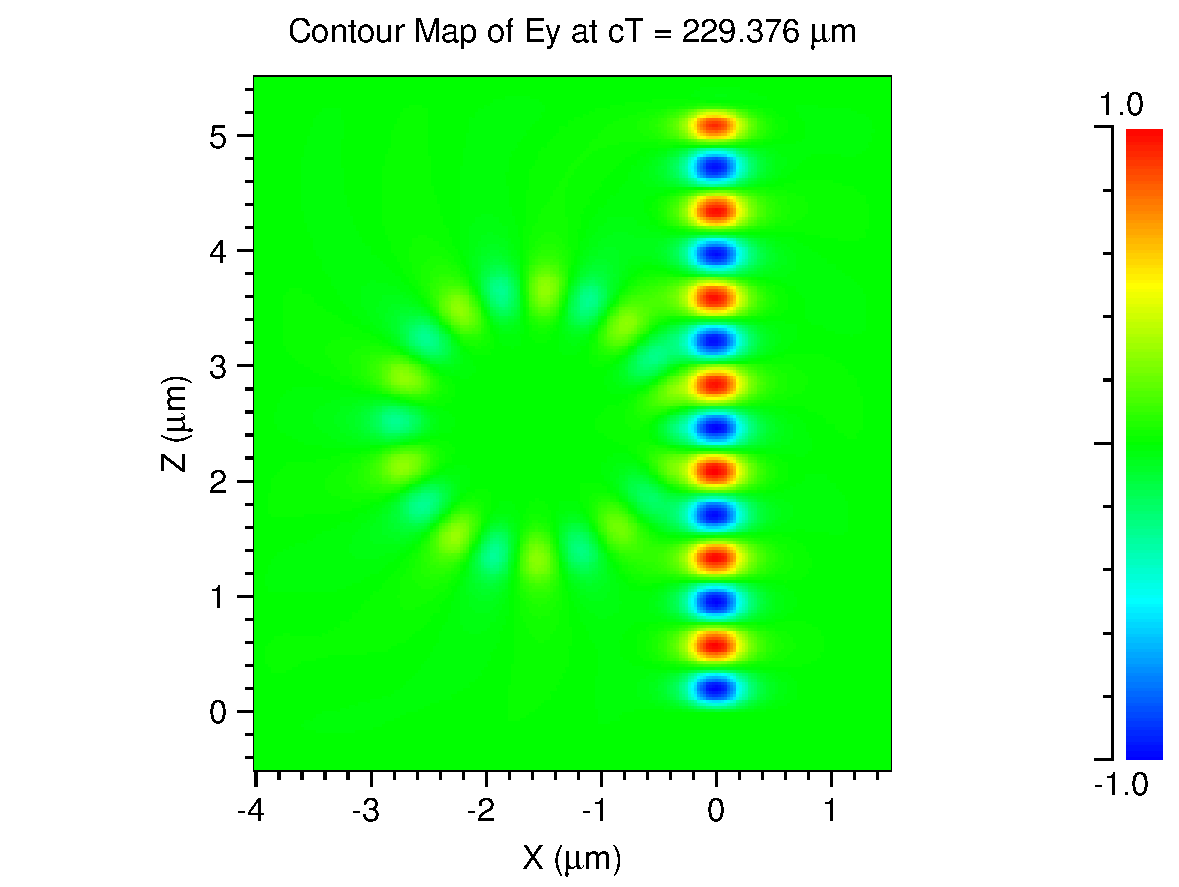
\includegraphics[totalheight=5 cm]{Grafiken/13_48_aufsicht.pdf}\label{fig:3_1_48_aufsicht}}
	\subfloat[]{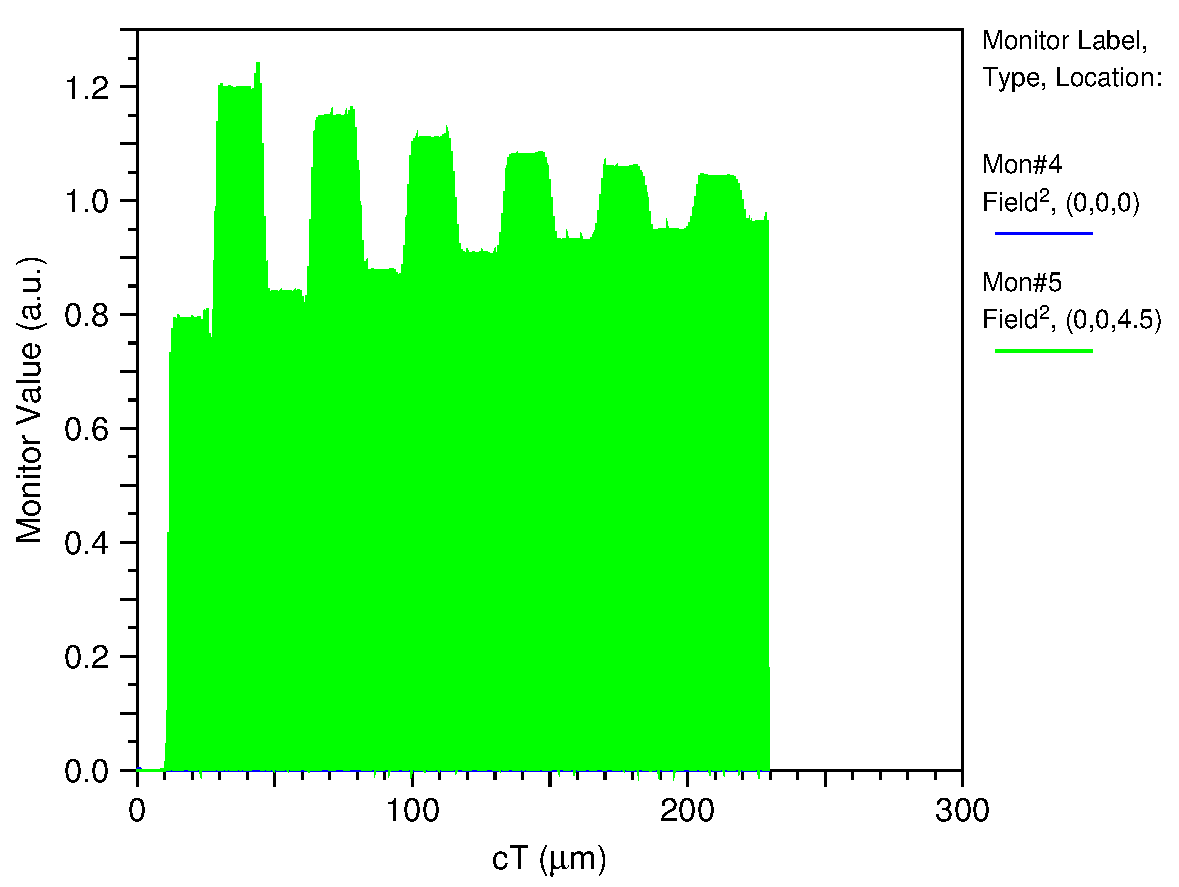
\includegraphics[totalheight=5 cm]{Grafiken/13_48_field.pdf} \label{fig:3_1_48_field}}\\%
\caption{Spatial Field Distribution \textbf{(a)} and Field at the Output \textbf{(b)} for a frequency of 202.7~THz}%
\label{fig:13_48}%
\end{figure}

\begin{figure}%
\centering
	\subfloat[]{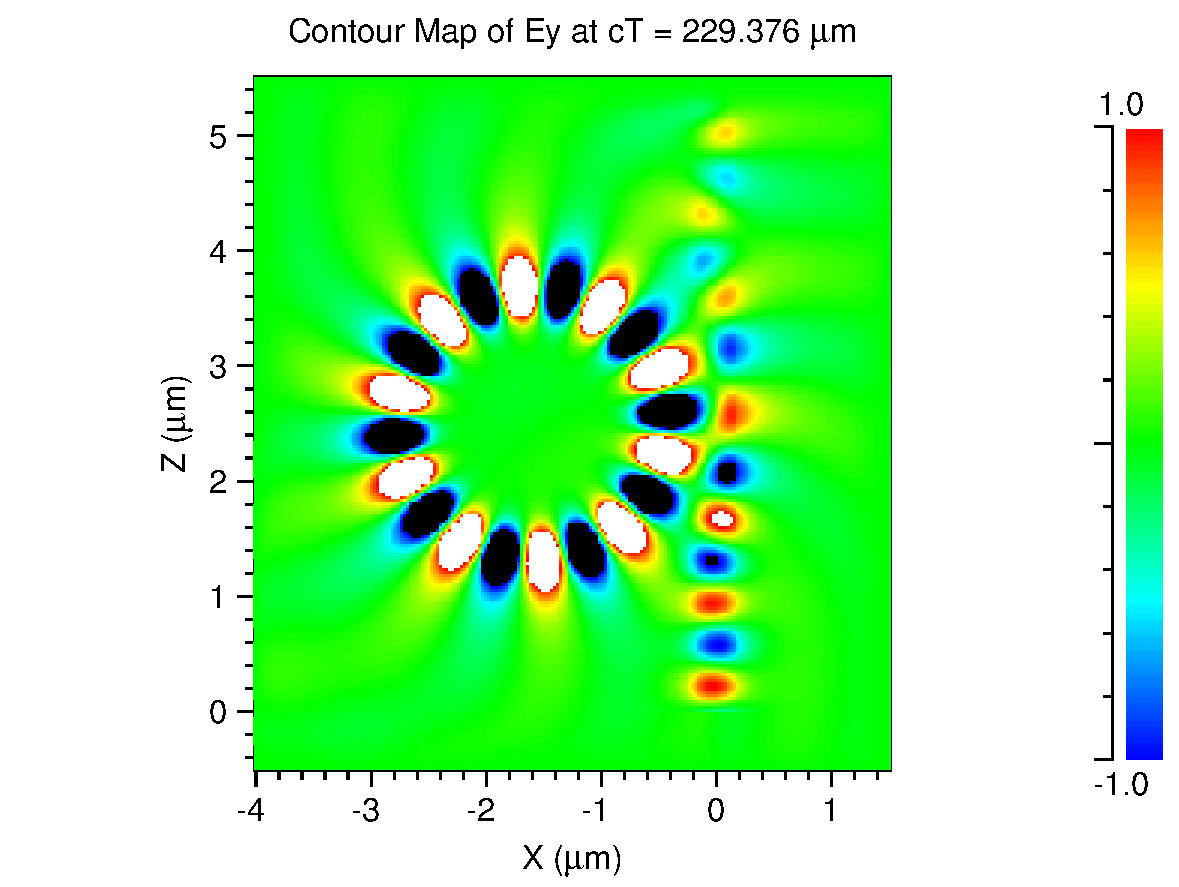
\includegraphics[totalheight=5 cm]{Grafiken/13_42_aufsicht.pdf}\label{fig:3_1_42_aufsicht}}
	\subfloat[]{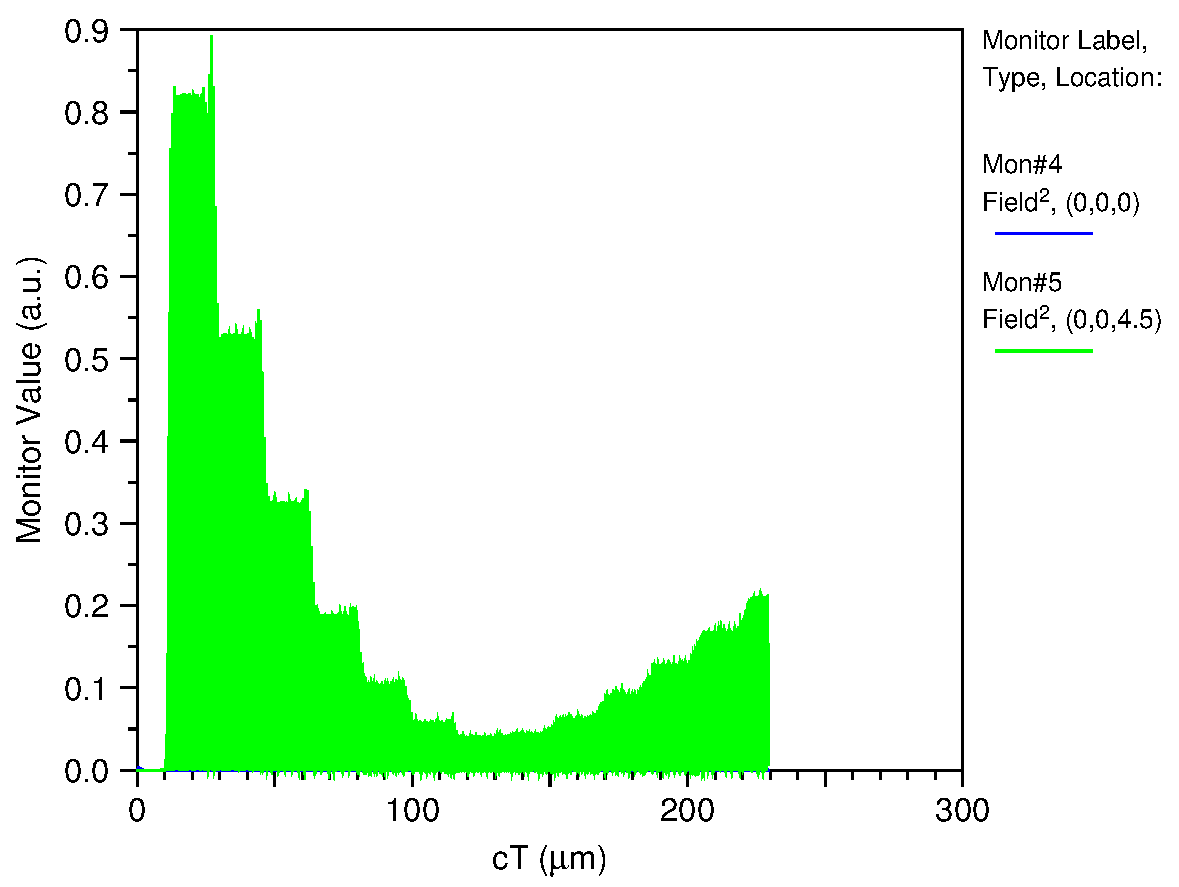
\includegraphics[totalheight=5 cm]{Grafiken/13_42_field.pdf} \label{fig:3_1_42_field}}\\%
\caption{Spatial Field Distribution \textbf{(a)} and Field at the Output \textbf{(b)} for a frequency of 211,5~THz}%
\label{fig:13_42}%
\end{figure}





% 
% \begin{table}%
% \centering
% \caption{Parameters of the first simulation}
% \begin{tabular}{lll}
% \toprule
% Exitation Type&Grid Size(x;y)&Stop Time\\
% ''Slab Mode``&(0.2;0.2)&32*1024*\\
% \bottomrule 
% \end{tabular}
% \label{tab:simulation1}
% \end{table}
At resonance the inserted power is stored in the ring. At resonance the condition \eqref{eq:res} is fulfilled and the field that is coupled into the resonantor and the field in the resonator interfere constructively. 

  
Although the attenuation in the resonator is zero there are losses inside the ring. This could be caused by the bend waveguide where the field is concentrated to the outer side of the bend waveguide. So parts of the field couple out of the bend waveguide and are radiating.
The experiment has additional attenuation in the waveguide. Therefore the losses are higher.

\newpage
One major difference between the simulation and the experiment is that the simulation calculates with an attenuation of zero which leads to differences in the transmission characteristic. Changing that simulation parameter is a possibility to better match the simulation with the experiment. 
Furthermore another simulation could be used. The beam propagation method uses the refractive index method which is a 2D simulation for a 3D structure. This reduces the computation time but leads to less accurate results. An alternative would be a 3D simulation with e.g. CST Microwave Studio. But the computation time for that would be much longer. 
